% Options for packages loaded elsewhere
% Options for packages loaded elsewhere
\PassOptionsToPackage{unicode}{hyperref}
\PassOptionsToPackage{hyphens}{url}
\PassOptionsToPackage{dvipsnames,svgnames,x11names}{xcolor}
%
\documentclass[
  spanish,
  a4paper,
  12pt,
  twoside]{memoir}
\usepackage{xcolor}
\usepackage{amsmath,amssymb}
\setcounter{secnumdepth}{-\maxdimen} % remove section numbering
\usepackage{iftex}
\ifPDFTeX
  \usepackage[T1]{fontenc}
  \usepackage[utf8]{inputenc}
  \usepackage{textcomp} % provide euro and other symbols
\else % if luatex or xetex
  \usepackage{unicode-math} % this also loads fontspec
  \defaultfontfeatures{Scale=MatchLowercase}
  \defaultfontfeatures[\rmfamily]{Ligatures=TeX,Scale=1}
\fi
\usepackage{lmodern}
\ifPDFTeX\else
  % xetex/luatex font selection
\fi
% Use upquote if available, for straight quotes in verbatim environments
\IfFileExists{upquote.sty}{\usepackage{upquote}}{}
\IfFileExists{microtype.sty}{% use microtype if available
  \usepackage[]{microtype}
  \UseMicrotypeSet[protrusion]{basicmath} % disable protrusion for tt fonts
}{}
\makeatletter
\@ifundefined{KOMAClassName}{% if non-KOMA class
  \IfFileExists{parskip.sty}{%
    \usepackage{parskip}
  }{% else
    \setlength{\parindent}{0pt}
    \setlength{\parskip}{6pt plus 2pt minus 1pt}}
}{% if KOMA class
  \KOMAoptions{parskip=half}}
\makeatother
% Make \paragraph and \subparagraph free-standing
\makeatletter
\ifx\paragraph\undefined\else
  \let\oldparagraph\paragraph
  \renewcommand{\paragraph}{
    \@ifstar
      \xxxParagraphStar
      \xxxParagraphNoStar
  }
  \newcommand{\xxxParagraphStar}[1]{\oldparagraph*{#1}\mbox{}}
  \newcommand{\xxxParagraphNoStar}[1]{\oldparagraph{#1}\mbox{}}
\fi
\ifx\subparagraph\undefined\else
  \let\oldsubparagraph\subparagraph
  \renewcommand{\subparagraph}{
    \@ifstar
      \xxxSubParagraphStar
      \xxxSubParagraphNoStar
  }
  \newcommand{\xxxSubParagraphStar}[1]{\oldsubparagraph*{#1}\mbox{}}
  \newcommand{\xxxSubParagraphNoStar}[1]{\oldsubparagraph{#1}\mbox{}}
\fi
\makeatother


\usepackage{longtable,booktabs,array}
\newcounter{none} % for unnumbered tables
\usepackage{calc} % for calculating minipage widths
% Correct order of tables after \paragraph or \subparagraph
\usepackage{etoolbox}
\makeatletter
\patchcmd\longtable{\par}{\if@noskipsec\mbox{}\fi\par}{}{}
\makeatother
% Allow footnotes in longtable head/foot
\IfFileExists{footnotehyper.sty}{\usepackage{footnotehyper}}{\usepackage{footnote}}
\makesavenoteenv{longtable}
\usepackage{graphicx}
\makeatletter
\newsavebox\pandoc@box
\newcommand*\pandocbounded[1]{% scales image to fit in text height/width
  \sbox\pandoc@box{#1}%
  \Gscale@div\@tempa{\textheight}{\dimexpr\ht\pandoc@box+\dp\pandoc@box\relax}%
  \Gscale@div\@tempb{\linewidth}{\wd\pandoc@box}%
  \ifdim\@tempb\p@<\@tempa\p@\let\@tempa\@tempb\fi% select the smaller of both
  \ifdim\@tempa\p@<\p@\scalebox{\@tempa}{\usebox\pandoc@box}%
  \else\usebox{\pandoc@box}%
  \fi%
}
% Set default figure placement to htbp
\def\fps@figure{htbp}
\makeatother



\ifLuaTeX
\usepackage[bidi=basic,shorthands=off]{babel}
\else
\usepackage[bidi=default,shorthands=off]{babel}
\fi
\ifLuaTeX
  \usepackage{selnolig} % disable illegal ligatures
\fi


\setlength{\emergencystretch}{3em} % prevent overfull lines

\providecommand{\tightlist}{%
  \setlength{\itemsep}{0pt}\setlength{\parskip}{0pt}}



 
\usepackage[]{natbib}
\bibliographystyle{apalike}


%% ============================================================
%%  Preámbulo LaTeX compartido – Memoria TFG GIS UBU
%%  Incluido automáticamente por memoria.qmd via include-before-body
%% ============================================================

% --- Clase y opciones ya las gestiona Quarto (memoir, a4paper, 12pt, twoside)

% --- Castellano
%\usepackage[spanish,es-tabla]{babel} % No es necesario en Quarto
%\selectlanguage{spanish} % No es necesario en Quarto
\addto\captionsspanish{\renewcommand{\tablename}{Tabla}}
\addto\captionsspanish{\renewcommand{\listtablename}{Índice de tablas}}
\addto\captionsspanish{\renewcommand{\contentsname}{Índice general}}
\addto\captionsspanish{\renewcommand{\listfigurename}{Índice de figuras}}


% --- Tipografía
\usepackage{lmodern}
\usepackage{microtype}
\usepackage{placeins}

% --- Tablas
\RequirePackage{booktabs}
%\RequirePackage[table]{xcolor}
\PassOptionsToPackage{table}{xcolor}
\RequirePackage{xtab}
\RequirePackage{multirow}
\RequirePackage{tabularx}

% --- Links
\PassOptionsToPackage{hyphens}{url}
\usepackage[colorlinks]{hyperref}
\hypersetup{allcolors={red}}

% --- Matemáticas
\usepackage{amsmath}

% --- Párrafos
\nonzeroparskip
\widowpenalty100000
\clubpenalty100000
\nouppercaseheads

% --- Márgenes espejo
\let\tmp\oddsidemargin
\let\oddsidemargin\evensidemargin
\let\evensidemargin\tmp
\reversemarginpar

% --- Imágenes
\usepackage{graphicx}
\graphicspath{{./img/}}

% --- Páginas en horizontal (para diagramas anchos)
\usepackage{pdflscape}

%% Comando \imagen{ruta}{caption}{escala}
\newcommand{\imagen}[3]{%
  \begin{figure}[!h]
    \centering
    \includegraphics[width=#3\textwidth]{#1}
    \caption{#2}\label{fig:#1}
  \end{figure}
  \FloatBarrier
}

%% Comando \ruta{texto}
\newcommand{\ruta}[1]{{\sffamily #1}}

% --- Estilo capítulos memoir
\chapterstyle{bianchi}

%% \capitulo{número}{título}  – capítulos sin numerar en el cuerpo
\newcommand{\capitulo}[2]{%
  \setcounter{chapter}{#1}%
  \setcounter{section}{0}%
  \setcounter{figure}{0}%
  \setcounter{table}{0}%
  \chapter*{#2}%
  \addcontentsline{toc}{chapter}{#2}%
  \markboth{#2}{#2}%
}

%% Apéndices
\renewcommand{\appendixname}{Apéndice}
\renewcommand*\cftappendixname{\appendixname}

\newcommand{\apendice}[1]{%
  \chapter{#1}%
}
\renewcommand*\cftappendixname{\appendixname\ }

% --- Portada personalizada UBU-GIS
\usepackage{xcolor}
\definecolor{newBox}{HTML}{D8AD6E}

\makeatletter
\newcommand{\tutor}[1]{\def\@tutor{#1}}
\newcommand{\tutorb}[1]{\def\@tutorb{#1}}
\newcommand{\tutorc}[1]{\def\@tutorc{#1}}
\newcommand{\course}[1]{\def\@course{#1}}

% ── EDITAR ESTOS DATOS ──────────────────────────────────────
\newcommand{\nombre}{Cristina Velázquez Romano}            % Tu nombre completo
\newcommand{\nombreTutor}{David García García}      % Nombre del tutor/a 1
\newcommand{\nombreTutorb}{Sergio Ossa Echeverri}     % Nombre del tutor/a 2
\newcommand{\nombreTutorc}{Rodrigo Albillos Almaraz}     % Nombre del tutor/a 3
\newcommand{\dni}{71310721A}                       % Tu DNI  
% ────────────────────────────────────────────────────────────

\tutor{\nombreTutor}
\tutorb{\nombreTutorb}
\tutorc{\nombreTutorc}

\def\maketitle{%
  \null
  \thispagestyle{empty}

\nouppercaseheads

\makepagestyle{mipc}
\makepsmarks{mipc}{%
  \nouppercaseheads
  \createmark{chapter}{both}{nonumber}{}{}
}
\makeevenhead{mipc}{\leftmark}{}{}   % páginas pares → izquierda
\makeoddhead{mipc}{}{}{\leftmark}    % páginas impares → derecha

\makeevenfoot{mipc}{}{\thepage}{}
\makeoddfoot{mipc}{}{\thepage}{}
\makeheadrule{mipc}{\textwidth}{\normalrulethickness}
\pagestyle{mipc}

\makepagestyle{chapterfirst}
\makeevenhead{chapterfirst}{}{}{}
\makeoddhead{chapterfirst}{}{}{}
\makeevenfoot{chapterfirst}{}{\thepage}{}
\makeoddfoot{chapterfirst}{}{\thepage}{}
\aliaspagestyle{chapter}{chapterfirst}

  % Cabecera
  \begin{center}
    \noindent
\includegraphics[width=\textwidth]{CabeceraEPS.png}\vspace{1.5cm}
  \end{center}
  % Logo GIS
  \begin{center}
    \begin{minipage}[c][1.5cm][c]{.20\textwidth}
      
\includegraphics[width=\textwidth]{Logo_GIS.png}
    \end{minipage}
  \end{center}
  % Caja título
  \begin{center}
    \colorbox{newBox}{%
      \begin{minipage}{.8\textwidth}
        \vspace{.5cm}\Large
        \begin{center}
          \textbf{TFG del Grado en Ingeniería de la Salud}\vspace{.6cm}\\
          \textbf{\LARGE\@title{}}
        \end{center}
        \vspace{.2cm}
      \end{minipage}
    }
  \end{center}
  % Datos
  \begin{center}
    \noindent\LARGE
    Presentado por \@author{}\\
    en Universidad de Burgos\\
    \vspace{0.5cm}
    \noindent\Large
    \@date{}\\
    \vspace{0.5cm}
    Tutores: \@tutor{} -- \@tutorb{} -- \@tutorc{}\\
  \end{center}
  \null
  \cleardoublepage
}
\makeatother
\makeatletter
\@ifpackageloaded{caption}{}{\usepackage{caption}}
\AtBeginDocument{%
\ifdefined\contentsname
  \renewcommand*\contentsname{Tabla de contenidos}
\else
  \newcommand\contentsname{Tabla de contenidos}
\fi
\ifdefined\listfigurename
  \renewcommand*\listfigurename{Listado de Figuras}
\else
  \newcommand\listfigurename{Listado de Figuras}
\fi
\ifdefined\listtablename
  \renewcommand*\listtablename{Listado de Tablas}
\else
  \newcommand\listtablename{Listado de Tablas}
\fi
\ifdefined\figurename
  \renewcommand*\figurename{Figura}
\else
  \newcommand\figurename{Figura}
\fi
\ifdefined\tablename
  \renewcommand*\tablename{Tabla}
\else
  \newcommand\tablename{Tabla}
\fi
}
\@ifpackageloaded{float}{}{\usepackage{float}}
\floatstyle{ruled}
\@ifundefined{c@chapter}{\newfloat{codelisting}{h}{lop}}{\newfloat{codelisting}{h}{lop}[chapter]}
\floatname{codelisting}{Listado}
\newcommand*\listoflistings{\listof{codelisting}{Listado de Listados}}
\makeatother
\makeatletter
\makeatother
\makeatletter
\@ifpackageloaded{caption}{}{\usepackage{caption}}
\@ifpackageloaded{subcaption}{}{\usepackage{subcaption}}
\makeatother
\usepackage{bookmark}
\IfFileExists{xurl.sty}{\usepackage{xurl}}{} % add URL line breaks if available
\urlstyle{same}
\hypersetup{
  pdftitle={Integración de señales BIS y variables clínicas para análisis retrospectivo en UCI},
  pdfauthor={Cristina Velázquez Romano},
  pdflang={es},
  colorlinks=true,
  linkcolor={blue},
  filecolor={Maroon},
  citecolor={Blue},
  urlcolor={Blue},
  pdfcreator={LaTeX via pandoc}}


\title{Integración de señales BIS y variables clínicas para análisis
retrospectivo en UCI}
\author{Cristina Velázquez Romano}
\date{}
\begin{document}
\frontmatter
\maketitle


\mainmatter
%% ── Datos de portada (editar aquí) ─────────────────────────
\title{Integración de señales BIS y variables clínicas para análisis retrospectivo en UCI}
\author{\nombre}
\date{\today}

\maketitle

%% ── Página de autorización (Vº Bº tutores) ─────────────────
\newpage\null\thispagestyle{empty}\newpage
\thispagestyle{empty}

\noindent
\includegraphics[width=\textwidth]{CabeceraEPS.png}\vspace{1cm}

\noindent D. \nombreTutor, profesor del departamento de Ingeniería Informática, área de Lenguajes y Sistemas Informáticos; D. Sergio Ossa Echeverri y D. Rodrigo Albillos Almaraz, tutores clínicos de la Unidad de Cuidados Intensivos, Hospital Universitario de Burgos.

\noindent Exponen:

\noindent Que la alumna Dña. \nombre, con DNI \dni, ha realizado el Trabajo
Fin de Grado en Ingeniería de la Salud titulado \textit{Integración de señales BIS y variables clínicas para análisis retrospectivo en UCI}.

\noindent Y que dicho trabajo ha sido realizado por la alumna bajo la
dirección del que suscribe, en virtud de lo cual se autoriza su presentación y defensa.

\begin{center}
  En Burgos, a {\large \today}
\end{center}

\vfill\vfill\vfill

\begin{minipage}{0.3\textwidth}
  \begin{flushleft}
    D. \nombreTutor
  \end{flushleft}
\end{minipage}
\hfill
\begin{minipage}{0.3\textwidth}
  \begin{flushleft}
    D. \nombreTutorb
  \end{flushleft}
\end{minipage}
\hfill
\begin{minipage}{0.3\textwidth}
  \begin{flushleft}
    D. \nombreTutorc
  \end{flushleft}
\end{minipage}

\vfill
\newpage\null\thispagestyle{empty}\newpage

%% ── Resumen / Abstract ──────────────────────────────────────
\frontmatter

\pagestyle{chapterfirst}

\renewcommand*\abstractname{Resumen}
\begin{abstract}
Este Trabajo Fin de Grado plantea una prueba de concepto orientada a la integración temporal y visualización conjunta de señales procedentes del monitor BIS y de variables clínicas extraídas del sistema ICCA en pacientes de la unidad de cuidados intensivos. El objetivo es facilitar el análisis retrospectivo de la evolución del paciente mediante la unificación de diferentes fuentes de información clínica y neurofisiológica en una misma línea temporal. Para ello, se aborda la extracción y organización de los datos por paciente y sesión, su normalización temporal, y el desarrollo de un visualizador interactivo que permita representar conjuntamente la matriz de densidad espectral, el índice BIS y variables clínicas seleccionadas.
\end{abstract}

\renewcommand*\abstractname{Descriptores}
\begin{abstract}
BIS, ICCA, unidad de cuidados intensivos, sincronización temporal, análisis retrospectivo, visualización de datos, prueba de concepto.
\end{abstract}

\clearpage

\renewcommand*\abstractname{Abstract}
\begin{abstract}
This Final Degree Project proposes a proof of concept focused on the temporal integration and joint visualization of signals from the BIS monitor and clinical variables extracted from the ICCA system in intensive care patients. The aim is to facilitate retrospective analysis of patient evolution by combining different clinical and neurophysiological data sources on a common timeline. To this end, the data are extracted and organized by patient and session, temporally normalized, and an interactive visualizer is developed to jointly display the density spectral array, BIS index and selected clinical variables.
\end{abstract}

\renewcommand*\abstractname{Keywords}
\begin{abstract}
BIS, ICCA, intensive care unit, temporal synchronization, retrospective analysis, data visualization, proof of concept.
\end{abstract}

\clearpage

\renewcommand{\contentsname}{Índice general}
\renewcommand{\listfigurename}{Índice de figuras}
\renewcommand{\listtablename}{Índice de tablas}

\tableofcontents
\clearpage
\listoffigures
\clearpage
\listoftables
\clearpage

\mainmatter

\pagestyle{mipc}

%% ── Capítulo 1: Introducción ────────────────────────────────
\capitulo{1}{Introducción}

La monitorización de los pacientes críticos en estado de sedación
ingresados en la Unidad de Cuidados Intensivos (UCI) requiere de la
integración de información procedente de múltiples dispositivos de
monitorización y otros sistemas clínicos con el fin de facilitar la toma
de decisiones, el seguimiento del paciente y el ajuste de la dosis
recibida por el mismo.

Entre estas fuentes de información, la monitorización neurofisiológica
mediante el índice biespectral o Bispectral Index (BIS) constituye una
herramienta de interés para valorar el estado de sedación a partir del
procesamiento de la actividad electroencefalográfica.

De forma complementaria, los sistemas de información clínica como el
IntelliSpace Critical Care \& Anesthesia (ICCA) permiten registrar
constantes vitales, parámetros analíticos, tratamientos administrados y
otra información relevante del paciente a lo largo del tiempo.

Sin embargo, en la práctica, la información procedente del monitor BIS
no siempre es comprendida por todos los profesionales, por lo que buena
parte del potencial de la herramienta no llega a aprovecharse
plenamente. Además, los datos obtenidos del BIS y la información clínica
recogida en ICCA no siempre se encuentran integrados de forma inmediata
o fácilmente explorables de manera conjunta. Esto dificulta el análisis
retrospectivo de la evolución del paciente, especialmente cuando se
pretende estudiar la relación temporal entre la señal neurofisiológica,
el índice BIS y otras variables clínicas, como constantes hemodinámicas,
parámetros metabólicos o la administración de fármacos.

En este contexto, surge la necesidad de disponer de una aproximación que
permita integrar ambas fuentes de información en una misma línea
temporal, de manera que sea posible observar de forma conjunta la
evolución del BIS y de variables clínicas relevantes. Esta necesidad es
especialmente relevante en el entorno de la UCI, donde la monitorización
continua, la heterogeneidad de los datos y la complejidad del estado
clínico del paciente hacen especialmente útil contar con herramientas
que faciliten la revisión estructurada de la información.

El presente Trabajo Fin de Grado se plantea como una prueba de concepto
orientada a la integración temporal y visualización conjunta de datos
procedentes del monitor BIS y del sistema ICCA. El trabajo no se enfoca
como el desarrollo de un producto software final, sino como una
aproximación inicial que permita estudiar la viabilidad de extraer,
sincronizar, estructurar y representar conjuntamente ambos tipos de
datos, sentando así una base para futuros desarrollos más avanzados.

La motivación principal del proyecto radica, por tanto, en la necesidad
de facilitar el análisis retrospectivo del paciente crítico mediante la
combinación de información neurofisiológica y clínica en un entorno
común de exploración. Para ello, se aborda el estudio de los datos
accesibles del monitor BIS, incluyendo la matriz de densidad espectral
(DSA) y el índice BIS, así como su integración con variables clínicas
seleccionadas procedentes de ICCA mediante estrategias de normalización
temporal.

En definitiva, este TFG desarrolla un sistema de organización,
reconstrucción y visualización retrospectiva que permite integrar la
actividad cerebral monitorizada mediante BIS con variables clínicas
extraídas de ICCA, manteniendo la trazabilidad de los datos originales y
respetando la naturaleza temporal de cada tipo de información.

\subsection{Estructura del documento}\label{estructura-del-documento}

La presente memoria se organiza en varios capítulos:

\textbf{Objetivos}: se definen las metas del trabajo, distinguiendo
entre el objetivo general, orientado a la integración y visualización
conjunta de datos BIS e ICCA, y los objetivos específicos que concretan
las tareas necesarias para alcanzarlo.

\textbf{Conceptos teóricos}: se ofrece la visión necesaria para
contextualizar el estudio, describiendo el fundamento del índice BIS y
de la monitorización neurofisiológica, el sistema ICCA y los conceptos
relacionados con el análisis espectral de señales EEG.

\textbf{Metodología}: se detalla el procedimiento seguido para el
desarrollo de la prueba de concepto, incluyendo la extracción y
organización de los datos BIS e ICCA, el flujo de reconstrucción de la
DSA, la estrategia de sincronización temporal entre ambas fuentes y las
herramientas empleadas en el desarrollo de las dos aplicaciones
propuestas.

\textbf{Resultados}: se presentan los resultados obtenidos, tanto en
relación con la reconstrucción de las variables BIS como con la
integración y visualización conjunta de los datos clínicos procedentes
de ICCA.

\textbf{Discusión}: se realiza un análisis crítico de los resultados
obtenidos y de las limitaciones del trabajo.

\textbf{Conclusiones}: se recogen las principales aportaciones del
proyecto y el grado de cumplimiento de los objetivos planteados.

\textbf{Líneas futuras}: una vez finalizado el proyecto, se proponen
posibles mejoras y ampliaciones para futuros desarrollos.

%% ── Capítulo 2: Objetivos ───────────────────────────────────
\capitulo{2}{Objetivos}

\section{Objetivo general}\label{objetivo-general}

Desarrollar una prueba de concepto para la integración y visualización
simultánea de datos procedentes del monitor BIS y de variables clínicas
extraídas del sistema ICCA, con el fin de facilitar su análisis
retrospectivo en el contexto de una unidad de cuidados intensivos.

\section{Objetivos específicos}\label{objetivos-especuxedficos}

\begin{enumerate}
\def\labelenumi{\arabic{enumi}.}
\tightlist
\item
  Caracterizar y organizar la información contenida en las diferentes
  exportaciones del monitor BIS y en las plantillas clínicas procedentes
  de ICCA, identificando los archivos, variables e intervalos temporales
  relevantes para el proyecto.
\item
  Diseñar una estrategia de organización de datos por paciente y sesión,
  que permita asociar registros BIS e información clínica
  correspondiente a un mismo periodo temporal.
\item
  Recuperar la matriz de densidad espectral proporcionada por el monitor
  BIS y permitir su reconstrucción a partir de la señal EEG cruda cuando
  el archivo espectral no exista o no contenga información válida.
\item
  Establecer una representación temporal común para la DSA y las
  variables procesadas del monitor, incluyendo el índice BIS, la
  frecuencia espectral de borde, la frecuencia mediana y, en los
  registros bilaterales, la asimetría entre hemisferios.
\item
  Integrar las variables clínicas procedentes de ICCA correspondientes
  al intervalo temporal de cada sesión BIS, respetando su resolución
  temporal y el instante real en el que fueron registradas.
\item
  Validar la fidelidad de la matriz de densidad espectral reconstruida
  frente a la matriz original del monitor, cuando esté disponible,
  mediante métricas de concordancia, como la correlación de Pearson,
  error absoluto medio (MAE) y raíz del error cuadrático medio (RMSE).
\item
  Desarrollar un visualizador interactivo que permita consultar
  registros BIS unilaterales y bilaterales, seleccionar diferentes
  intervalos temporales y representar conjuntamente la DSA, los
  parámetros procesados del BIS y la información clínica disponible.
\end{enumerate}

\section{Objetivos de aprendizaje}\label{objetivos-de-aprendizaje}

Además de los objetivos técnicos del proyecto, este trabajo persigue una
serie de objetivos formativos relacionados con las competencias propias
del Grado en Ingeniería de la Salud. Entre ellos destacan:

\begin{itemize}
\tightlist
\item
  Comprender el funcionamiento básico del monitor BIS y la naturaleza de
  las señales asociadas a la monitorización neurofisiológica.
\item
  Afianzar los conceptos fundamentales del tratamiento de señales
  biomédicas, incluyendo la representación temporal de una señal, su
  análisis en el dominio de la frecuencia y la interpretación de
  magnitudes como amplitud, frecuencia, potencia y densidad espectral.
\item
  Profundizar en el análisis del electroencefalograma y en su
  representación mediante herramientas frecuenciales, como el espectro
  de potencia y la matriz de densidad espectral.
\item
  Profundizar en el tratamiento, organización y análisis de datos
  biomédicos heterogéneos.
\item
  Aplicar estrategias de sincronización temporal y estructuración de
  datos clínicos procedentes de distintas fuentes.
\item
  Desarrollar una prueba de concepto orientada a una necesidad real del
  entorno clínico.
\item
  Fortalecer la capacidad de documentación técnica, planificación y
  desarrollo de proyectos en el ámbito de la ingeniería de la salud.
\end{itemize}

%% ── Capítulo 3: Marco teórico ───────────────────────────────
\capitulo{3}{Conceptos teóricos}

En esta sección se presentan los conceptos fundamentales necesarios para
comprender el contexto clínico y técnico del trabajo.

\section{Unidad de cuidados intensivos (UCI) y monitorización del
paciente
crítico}\label{unidad-de-cuidados-intensivos-uci-y-monitorizaciuxf3n-del-paciente-cruxedtico}

La unidad de cuidados intensivos (UCI) es un área hospitalaria altamente
especializada destinada a la atención de pacientes con patologías graves
o con riesgo vital, que requieren de una vigilancia estrecha y soporte
continuo.

En este entorno, la inestabilidad fisiológica de los pacientes exige una
monitorización continua y exhaustiva de múltiples parámetros clínicos.
Dentro del manejo habitual, la administración de fármacos sedantes y
analgésicos constituye una práctica frecuente, orientada a reducir el
estrés metabólico, facilitar la adaptación a la ventilación mecánica y
evitar el dolor. En consecuencia, el control adecuado del nivel de
sedación resulta fundamental, ya que una dosificación insuficiente o
excesiva puede influir de forma directa en la evolución clínica. En
particular, la sobresedación, entendida como la administración de una
cantidad de sedantes superior a la estrictamente necesaria, se ha
asociado con un aumento de la morbilidad y la mortalidad. Un exceso de
sedación puede prolongar el tiempo de ventilación mecánica, retrasar el
despertar y aumentar el riesgo de complicaciones asociadas, como la
neumonía, contribuyendo además a una mayor estancia en la UCI
\citep{chamorro2008}.

\section{Electroencefalograma (EEG) y
ondas}\label{electroencefalograma-eeg-y-ondas}

El electroencefalograma (EEG) es una prueba que registra la actividad
eléctrica cerebral mediante electrodos colocados sobre el cuero
cabelludo \citep{medlineplusEEG}. La señal obtenida refleja diferencias
de potencial entre electrodos, organizadas en canales de registro, y
procede principalmente de la actividad sincrónica de grandes poblaciones
de neuronas corticales, especialmente de las dendritas de las neuronas
piramidales \citep{Louis2016A1}. Una de las principales ventajas del EEG
es su elevada resolución temporal, del orden de milisegundos, lo que
permite estudiar cambios rápidos en la actividad cerebral
\citep{Louis2016A2}.

\subsection{Amplitud, frecuencia, potencia, densidad espectral y
decibelios.}\label{amplitud-frecuencia-potencia-densidad-espectral-y-decibelios.}

En el ámbito del procesamiento de señales, la actividad
electroencefalográfica se describe mediante los siguientes conceptos
\citep{Kane2017}:

\begin{itemize}
\item
  Ciclo: oscilación completa de una onda, desde un punto inicial hasta
  que vuelve a alcanzar el mismo estado tras pasar por un máximo
  (cresta) y un mínimo (valle).
\item
  Amplitud: magnitud de la variación de la señal respecto a un valor de
  referencia. En el EEG se expresa habitualmente en microvoltios (µV).
\item
  Frecuencia: número de ciclos que se producen por segundo. Se expresa
  en hercios (Hz).
\item
  Potencia de la señal: magnitud empleada en procesamiento de señales
  para cuantificar el valor cuadrático medio de sus oscilaciones. Como
  la amplitud del EEG se expresa en microvoltios, la potencia de señal
  se expresa en microvoltios al cuadrado (\(\mu\mathrm{V}^2\))
  \citep{OppenheimSchafer2014}.\footnote{Esta magnitud describe
    matemáticamente la señal y no debe confundirse con la potencia
    eléctrica físicamente transferida o consumida, que se expresaría en
    vatios.}
\item
  Densidad espectral de potencia: indica cómo se distribuye la potencia
  de la señal entre las distintas frecuencias, expresada en µV²/Hz. Al
  integrar esta densidad dentro de un intervalo de frecuencias se
  obtiene la potencia contenida en esa banda, expresada en µV².
\item
  Decibelios (dB): escala logarítmica que expresa la potencia respecto a
  un valor de referencia. Para construir la matriz de densidad espectral
  (DSA), la potencia calculada en cada intervalo frecuencial se
  transforma a decibelios mediante una comparación logarítmica con una
  potencia de referencia. Dicha referencia se obtiene elevando al
  cuadrado la amplitud de 0,0001 µV RMS (Root Mean Square, valor eficaz
  o cuadrático medio de la señal) \citep{CovidienSerial2010} indicada
  por el fabricante (resultando en \(10^{-8}\) µV²).
\end{itemize}

\subsection{Espectro y espectrograma}\label{espectro-y-espectrograma}

El EEG puede analizarse tanto en el dominio temporal como en el
frecuencial \citep{Kane2017}. Mientras que en el dominio temporal se
observa cómo varía la amplitud de la señal a lo largo del tiempo, el
análisis frecuencial permite identificar cómo se distribuye su potencia
entre las distintas frecuencias y bandas.

El espectro de potencia representa la potencia contenida en cada
frecuencia durante un intervalo de tiempo determinado. Permite reconocer
qué componentes frecuenciales predominan, pero no muestra cómo cambian a
lo largo del registro.

El espectrograma amplía este análisis calculando sucesivos espectros
sobre intervalos temporales consecutivos. El resultado es una
representación tiempo-frecuencia en la que un eje muestra el tiempo,
otro la frecuencia y el color indica la potencia de la señal. De esta
forma, permite observar la evolución del contenido espectral del EEG e
identificar cambios en el predominio de determinadas bandas
\citep{Ng2022}.

En este trabajo, esta representación constituye la base de la matriz de
densidad espectral empleada por el monitor BIS. Su procedimiento
concreto de cálculo y reconstrucción se describe en el capítulo de
metodología.

\subsection{Electroencefalografía
cuantitativa}\label{electroencefalografuxeda-cuantitativa}

La electroencefalografía cuantitativa (qEEG) hace referencia al conjunto
de técnicas que permiten analizar la señal EEG mediante métodos
numéricos y computacionales \citep{Hwang2022}. A diferencia de la
interpretación visual convencional del trazado, el qEEG permite extraer
parámetros objetivos relacionados con la amplitud, la frecuencia, la
potencia o la distribución espectral de la señal.

En el contexto de la monitorización cerebral, estas técnicas permiten
resumir grandes volúmenes de señal EEG en variables más interpretables,
como la potencia por bandas de frecuencia, la frecuencia de borde
espectral, la frecuencia mediana, la tasa de supresión o
representaciones tiempo-frecuencia como la matriz de densidad espectral
\citep{Hwang2022, Ng2022}. Por ello, el qEEG constituye la base técnica
de muchos parámetros mostrados por monitores como el BIS.

\subsubsection{Transformada de Fourier y análisis
frecuencial}\label{transformada-de-fourier-y-anuxe1lisis-frecuencial}

El análisis frecuencial de una señal se basa en descomponer su evolución
temporal en componentes sinusoidales caracterizadas por su frecuencia,
amplitud y fase. La transformada de Fourier permite pasar del dominio
temporal, donde se observa la evolución de la amplitud en el tiempo, al
dominio frecuencial, donde se estudia qué frecuencias están presentes en
la señal y con qué peso relativo \citep{OppenheimSchafer2014}.

En señales digitales, como el EEG registrado por el monitor BIS, no se
dispone de una función continua sino de una secuencia finita de
muestras. Por ello se emplea la transformada discreta de Fourier (DFT),
que calcula un conjunto finito de coeficientes frecuenciales a partir de
una ventana de señal. Cada coeficiente es un número complejo cuya
magnitud se relaciona con la amplitud de una determinada componente
frecuencial, mientras que su ángulo representa la fase
\citep{OppenheimSchafer2014}.

En la práctica, la DFT suele calcularse mediante la transformada rápida
de Fourier (FFT), que no es una transformada diferente, sino un
algoritmo eficiente para obtener el mismo resultado con menor coste
computacional \citep{OppenheimSchafer2014}. En el análisis de EEG, este
tipo de procesamiento permite calcular los componentes frecuenciales de
señales EEG digitalizadas y construir representaciones espectrales como
el espectrograma \citep{Sawa2022}.

\subsubsection{Estimación espectral mediante el método de
Welch}\label{estimaciuxf3n-espectral-mediante-el-muxe9todo-de-welch}

La aplicación directa de la DFT a una única ventana de señal permite
obtener una estimación del contenido frecuencial, pero esta estimación
puede ser sensible al ruido y a las características concretas del
segmento analizado. Para obtener una estimación más estable de la
densidad espectral de potencia se puede emplear el método de Welch
\citep{Welch1967, OppenheimSchafer2014}.

Este método consiste en dividir la señal en ventanas temporales más
cortas, normalmente con cierto solapamiento entre ellas. A cada ventana
se le aplica una función de ponderación, como una ventana de Hann, para
reducir los efectos de borde. Posteriormente se calcula el espectro de
potencia de cada segmento mediante la FFT y se promedian las
estimaciones obtenidas.

El resultado es una estimación de la densidad espectral de potencia
menos variable que la obtenida a partir de un único periodograma. En el
análisis de señales EEG, este enfoque resulta útil porque permite
estudiar cómo se distribuye la potencia de la señal entre las distintas
frecuencias. Cuando este procedimiento se aplica de forma sucesiva a lo
largo del tiempo, permite construir representaciones tiempo-frecuencia
como las empleadas en los espectrogramas y en la reconstrucción de la
DSA.

\subsection{Tipos de ondas del EEG}\label{tipos-de-ondas-del-eeg}

Para sistematizar la interpretación clínica de este contenido espectral,
las oscilaciones del EEG se clasifican habitualmente en distintas bandas
estandarizadas según el rango de frecuencias en el que oscilan las ondas
que las componen. Las principales bandas y su significado fisiológico
general se recogen en la Tabla~\ref{tbl-bandas-eeg}.

\begin{longtable}[]{@{}lrl@{}}
\caption{Bandas de frecuencia del EEG y asociaciones generales.
Elaboración propia a partir de
\citet{Er2006}.}\label{tbl-bandas-eeg}\tabularnewline
\toprule\noalign{}
Tipo de onda & Rango de frecuencia (Hz) & Interpretación general \\
\midrule\noalign{}
\endfirsthead
\toprule\noalign{}
Tipo de onda & Rango de frecuencia (Hz) & Interpretación general \\
\midrule\noalign{}
\endhead
\bottomrule\noalign{}
\endlastfoot
Gamma & \textgreater30 & Actividad rápida \\
Beta & 12--30 & Estado de alerta o activación \\
Alfa & 8--12 & Vigilia relajada, escasa actividad mental \\
Theta & 4--8 & Somnolencia o menor nivel de alerta \\
Delta & 1--4 & Sueño profundo o sedación intensa \\
\end{longtable}

El predominio de las distintas bandas y las características del EEG
varían según la edad, el estado clínico, el nivel de consciencia, el
ciclo sueño-vigilia, la apertura ocular y los fármacos administrados.
Además, deben distinguirse los cambios fisiológicos de los artefactos y
de posibles alteraciones patológicas. Por ello, el registro de estas
ondas no debe interpretarse de manera aislada, sino considerando las
condiciones en las que fue obtenido y el contexto clínico del paciente
\citep{Er2006}. El análisis asistido por software permite cuantificar la
potencia de las distintas bandas y representarla mediante herramientas
como la matriz de densidad espectral \citep{Tatum2016}.

\section{Monitor BIS}\label{monitor-bis}

\subsection{Monitor e Índice Biespectral
(BIS)}\label{monitor-e-uxedndice-biespectral-bis}

El monitor BIS\texttrademark{} es el dispositivo de neuromonitorización,
fabricado por Covidien (actualmente Medtronic), que adquiere y procesa
de forma continua las señales electroencefalográficas (EEG) frontales
del paciente mediante un sensor conectado a un módulo BISx o BISx4
\citep{CovidienBISadvanced}. Es, por tanto, el equipo físico: la
pantalla, el procesador y el módulo de adquisición, no un valor ni una
medida en sí mismo.

En este trabajo se han empleado datos procedentes de dos versiones del
equipo, BIS VISTA y BIS Advance, que comparten los mismos fundamentos de
adquisición y procesamiento de la señal, aunque presentan diferencias de
hardware e interfaz \citep{CovidienBISadvanced}. La estructura de los
archivos exportados por ambos equipos, prácticamente equivalente entre
versiones, se detalla en el Anexo F.

\begin{figure}

\centering{

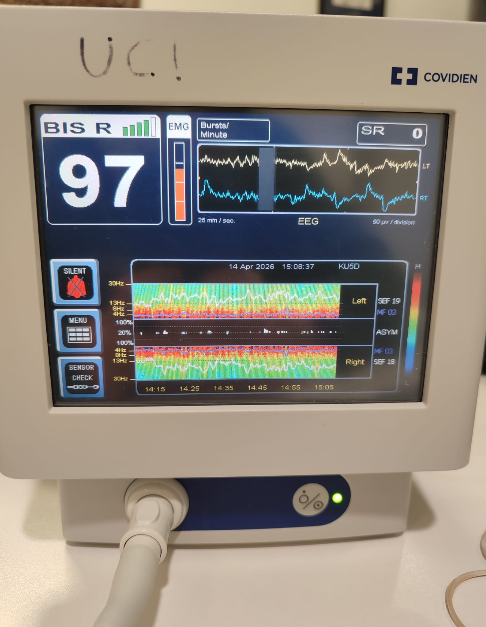
\includegraphics[width=0.45\linewidth,height=\textheight,keepaspectratio]{img/bis_vista.png}

}

\caption{\label{fig-monitor-vista}Monitor BIS VISTA. Fuente: Elaboración
propia \citep{CovidienBISadvanced}.}

\end{figure}%

\begin{figure}

\centering{

\includegraphics[width=0.45\linewidth,height=\textheight,keepaspectratio]{img/bis_Advance.png}

}

\caption{\label{fig-monitor-advance}Monitor BIS Advance. Fuente:
Elaboración propia \citep{CovidienBISadvanced}.}

\end{figure}%

A partir de la señal EEG adquirida, el monitor calcula y muestra en
pantalla un conjunto de parámetros procesados, entre los que se
encuentra el índice BIS descrito a continuación, junto con la matriz de
densidad espectral (DSA), la frecuencia de borde espectral (SEF), la
frecuencia mediana (MEF) y otros parámetros que se describen más
adelante en este capítulo.

\subsection{Matriz de densidad espectral
(DSA)}\label{matriz-de-densidad-espectral-dsa}

La matriz de densidad espectral o Density Spectral Array (DSA) es la
representación tipo espectrograma empleada por el monitor BIS para
mostrar la evolución de la potencia espectral del EEG
\citep{OchoaSolana2025}. Su interpretación se basa en los principios
descritos anteriormente: permite reconocer el predominio y la evolución
de las distintas bandas de frecuencia a partir del mapa de colores.

Desde el punto de vista clínico, la DSA facilita la identificación de
patrones o «firmas espectrales» asociados a determinados fármacos y
estados de consciencia \citep{LpezCastruita2023}. Por ejemplo, durante
la anestesia general con propofol puede observarse actividad lenta entre
0,5 y 1 Hz junto con una concentración de potencia alfa frontal,
aproximadamente entre 9 y 12 Hz \citep{LpezCastruita2023}. No obstante,
estos patrones deben interpretarse junto con la situación clínica y el
resto de los parámetros disponibles.

\subsection{Frecuencia del Borde Espectral y Frecuencia
Mediana}\label{frecuencia-del-borde-espectral-y-frecuencia-mediana}

Para complementar la información de la DSA, el monitor calcula
parámetros que resumen la distribución de la potencia en el dominio
frecuencial \citep{OchoaSolana2025}:

\begin{itemize}
\item
  \textbf{Frecuencia del Borde Espectral (SEF, Spectral Edge
  Frequency):} Representada habitualmente como la SEF95, indica la
  frecuencia por debajo de la cual se encuentra el 95 \% de la potencia
  total del EEG \citep{OchoaSolana2025}. En la DSA se dibuja como una
  línea blanca.
\item
  \textbf{Frecuencia Mediana (MF, Median Frequency):} Indica la
  frecuencia que divide la potencia del espectro en dos mitades exactas
  (50 \% por encima y 50 \% por debajo), trazándose en el espectrograma
  como una línea púrpura. Ambos parámetros permiten resumir el
  desplazamiento del contenido espectral del EEG, la disminución de los
  mismos refleja un predominio de frecuencias más lentas, aunque su
  interpretación depende del fármaco administrado, la profundidad de la
  sedación y la situación clínica del paciente \citep{OchoaSolana2025}.
\end{itemize}

\subsection{Electromiograma (EMG)}\label{electromiograma-emg}

El indicador electromiográfico (EMG) del monitor BIS refleja la potencia
registrada en la banda de 70 a 110 Hz. Esta banda contiene
principalmente actividad muscular frontal, aunque también puede incluir
otras interferencias de alta frecuencia \citep{SaboyaSnchez2009}.

Clínicamente, un aumento de la actividad muscular interfiere con la
captura de la señal EEG pura y provoca una elevación artificial del
número BIS, sugiriendo un nivel de consciencia mayor al real
\citep{SaboyaSnchez2009}. Esta sobreestimación desaparece al administrar
fármacos bloqueantes neuromusculares (BNM), por tanto, la ausencia de
señal EMG en el monitor otorga una mayor fiabilidad a los índices de
profundidad anestésica mostrados \citep{SaboyaSnchez2009}.

\subsection{Supresión de ráfagas
(SR)}\label{supresiuxf3n-de-ruxe1fagas-sr}

El patrón de brote-supresión (burst-suppression) refleja un estado de
depresión cortical profunda, caracterizado por ráfagas de actividad
eléctrica de alto voltaje seguidas de periodos de supresión del EEG o
silencio isoeléctrico casi absoluto \citep{OchoaSolana2025}. Este patrón
surge en contextos de anestesia profunda, hipotermia o daño cerebral
severo \citep{OchoaSolana2025}.

El monitor sintetiza este fenómeno mediante la Tasa de Supresión o
Suppression Ratio (SR), que expresa el porcentaje de tiempo, dentro de
una ventana temporal reciente (de unos 63 segundos)
\citep{CovidienBISadvanced}, en el que la señal EEG se considera
suprimida.

Una SR elevada indica una presencia relevante de periodos de supresión
y, por tanto, debe interpretarse como un posible marcador de depresión
cortical intensa. En el contexto de este trabajo, este parámetro resulta
útil para complementar la interpretación del índice BIS y de la DSA,
especialmente en registros con sedación profunda o alteraciones
neurológicas \citep{OchoaSolana2025}.

\subsection{Calidad de la señal (SQI) y
artefactos}\label{calidad-de-la-seuxf1al-sqi-y-artefactos}

El Índice de Calidad de la Señal o Signal Quality Index (SQI) evalúa la
fiabilidad del registro electroencefalográfico. De forma general,
expresa el porcentaje de señal que el algoritmo considera válida para el
cálculo de los parámetros mostrados, teniendo en cuenta la presencia de
artefactos, ruido o problemas de adquisición \citep{SaboyaSnchez2009}.

La calidad del EEG puede verse afectada por distintos factores, como un
mal contacto de los electrodos, movimientos del paciente, interferencias
eléctricas, actividad muscular o desplazamientos del sensor. Cuando el
SQI disminuye, la interpretación del índice BIS y del resto de variables
derivadas debe realizarse con cautela, ya que los valores mostrados
pueden no reflejar adecuadamente la actividad cerebral real.

En el contexto de este trabajo, el SQI resulta especialmente relevante
porque permite valorar la fiabilidad de los tramos analizados y detectar
periodos en los que las señales reconstruidas o visualizadas pueden
estar condicionadas por problemas de adquisición.

\section{Sistema IntelliSpace Critical Care \& Anesthesia (ICCA) y
registro de variables
clínicas}\label{sistema-intellispace-critical-care-anesthesia-icca-y-registro-de-variables-cluxednicas}

ICCA es un sistema de información clínica empleado en entornos de
cuidados críticos y anestesia para centralizar información generada
durante la atención del paciente. Este tipo de sistemas permite reunir
datos procedentes de monitores, dispositivos médicos y registros
clínicos realizados por el personal sanitario \citep{Lai2022}.

En la UCI, esta información resulta especialmente útil para reconstruir
el contexto clínico en el que se producen determinados cambios
fisiológicos o terapéuticos. Además, distintos estudios han utilizado
datos extraídos de ICCA para realizar análisis retrospectivos de
variables clínicas continuas, como frecuencia cardiaca o presión
arterial, en pacientes críticos \citep{Laichinger2024, Mengel2025}.

En este trabajo, ICCA se considera la fuente principal de información
clínica complementaria a la neuromonitorización BIS. Estas variables
permiten interpretar la señal electroencefalográfica y los parámetros
derivados del EEG dentro del contexto clínico real del paciente.

\section{Estado del arte y trabajos
relacionados}\label{estado-del-arte-y-trabajos-relacionados}

\subsection{Reconstrucción y visualización de DSA en monitorización
EEG/BIS}\label{reconstrucciuxf3n-y-visualizaciuxf3n-de-dsa-en-monitorizaciuxf3n-eegbis}

La qEEG ha sido esencial en cuidados críticos para transformar registros
EEG prolongados en representaciones más compactas e interpretables.
Hwang et al.~revisan distintas aplicaciones del qEEG en UCI adulta y
destacan el uso de representaciones como la CDSA (Color Density Spectral
Array) o la qEEG para facilitar la revisión visual de registros
extensos, reduciendo la necesidad de analizar de forma continua el EEG
crudo \citep{Hwang2022}. Estas herramientas permiten identificar cambios
en el contenido espectral de la señal y resumir la evolución de la
actividad cerebral en el tiempo.

En el ámbito de la anestesia, también se han desarrollado trabajos
orientados a analizar el EEG mediante espectrogramas generados
computacionalmente. Por ejemplo, Sawa et al.~presentan una aproximación
basada en Python para calcular y visualizar el espectro de potencia y el
espectrograma del EEG durante anestesia general, mostrando cómo el
procesamiento digital permite representar la evolución frecuencial de la
señal de forma interpretable \citep{Sawa2022}. Este tipo de trabajos
resulta cercano al presente TFG, ya que la reconstrucción de la DSA
requiere transformar señales EEG en representaciones tiempo-frecuencia.

No obstante, gran parte de estos trabajos se centran en el análisis
general del EEG o en la interpretación clínica del qEEG, pero no en la
reconstrucción práctica de la DSA a partir de archivos exportados por un
monitor BIS. En este contexto, el presente trabajo aporta una aplicación
orientada a reconstruir, visualizar y explorar registros BIS, incluyendo
la DSA, parámetros derivados y diferencias entre registros unilaterales
y bilaterales.

\subsection{Dashboards interactivos e integración de datos clínicos en
UCI}\label{dashboards-interactivos-e-integraciuxf3n-de-datos-cluxednicos-en-uci}

De forma paralela, distintos trabajos han abordado la necesidad de
integrar y visualizar grandes volúmenes de información clínica en UCI.
Las revisiones sobre dashboards clínicos señalan que los profesionales
deben interpretar simultáneamente constantes vitales, parámetros
ventilatorios, tratamientos, analíticas, alarmas y observaciones
clínicas, lo que puede aumentar la carga cognitiva y dificultar la
identificación rápida de cambios relevantes
\citep{Khairat2018, Wright2019}.

En este contexto, se han propuesto herramientas visuales orientadas a
reorganizar la información del paciente crítico. MIVA 2.0, por ejemplo,
se diseñó como un dashboard centrado en el usuario para facilitar la
revisión rápida de tendencias fisiológicas \citep{Faiola2015}. Por su
parte, el i-Dashboard integró información procedente de ICCA, HIS, LIS y
PACS para apoyar las rondas multidisciplinares en UCI, reduciendo el
tiempo dedicado a recopilar datos y mejorando la comunicación clínica
\citep{Lai2022}.

También existen sistemas más orientados a la adquisición y análisis de
datos multimodales. INSMA permite recoger ondas fisiológicas, alarmas y
variables numéricas procedentes de monitores Philips IntelliVue, además
de revisar datos históricos en ventanas temporales seleccionadas
\citep{Sun2020}. Otros trabajos han planteado infraestructuras de
almacenamiento de datos de alta frecuencia para facilitar el análisis
retrospectivo de señales de UCI \citep{Noteboom2024}.

Estos antecedentes muestran el interés creciente por integrar señales
fisiológicas y variables clínicas en herramientas visuales. Sin embargo,
la mayoría de las soluciones revisadas se centran en dashboards
generales de UCI, adquisición multimodal o análisis retrospectivo
amplio, sin abordar de forma específica la visualización conjunta de
registros BIS/DSA con variables clínicas complementarias. Por ello, el
presente trabajo se sitúa en la intersección entre la reconstrucción de
neuromonitorización BIS y el diseño de herramientas visuales para el
análisis retrospectivo contextualizado del paciente crítico.

%% ── Capítulo 4: Metodología ─────────────────────────────────
\capitulo{4}{Metodología}

\section{Enfoque general del
proyecto}\label{enfoque-general-del-proyecto}

El proyecto se plantea como una prueba de concepto orientada a la
integración temporal y visualización conjunta de información procedente
del monitor BIS y de variables clínicas registradas en ICCA. El objetivo
no es desarrollar un producto clínico final ni sustituir la
interpretación médica, sino estudiar la viabilidad de organizar,
sincronizar y representar ambas fuentes de información para facilitar el
análisis retrospectivo de pacientes críticos.

Para ello se diseñaron dos flujos de trabajo complementarios. El primero
permite organizar los datos disponibles por paciente y por sesión BIS,
asociando a cada registro neurofisiológico la información clínica
correspondiente. El segundo permite visualizar de forma conjunta la
matriz de densidad espectral, las variables procesadas del monitor BIS y
las variables clínicas seleccionadas procedentes de ICCA.

El proyecto se ha desarrollado con datos reales procedentes del Hospital
Universitario de Burgos (HUBU), cuyo uso fue autorizado por el Comité de
Bioética correspondiente. El detalle de esta aprobación y de las
condiciones bajo las que se ha tratado la información se recoge en el
Anexo F.

\section{Fuentes de datos utilizadas}\label{fuentes-de-datos-utilizadas}

\subsection{Datos BIS}\label{datos-bis}

Los datos del monitor BIS proceden de las exportaciones generadas por
los equipos BIS VISTA y BIS Advance
\citep{CovidienBISadvanced, CovidienSerial2010}. En este trabajo se
emplean principalmente los archivos \texttt{.spa}, \texttt{.f\_a},
\texttt{.r2a} o \texttt{.r4a}, \texttt{.h\_a} y \texttt{.t\_a},
explicados con detalle en el Anexo F:

\begin{itemize}
\item
  El archivo \texttt{.spa} contiene las variables procesadas por el
  monitor, como el índice BIS, SEF, MEF, SQI y otros parámetros de
  configuración.
\item
  El archivo \texttt{.f\_a} contiene la matriz espectral calculada por
  el propio monitor. Este archivo no siempre está disponible, ya que el
  equipo BIS VISTA lo exporta vacío.
\item
  La cabecera \texttt{.h\_a} proporciona la pendiente y el offset,
  información de calibración necesaria para convertir los valores crudos
  a microvoltios.
\item
  El archivo \texttt{.t\_a} aporta el instante en el que comienza el BIS
  a registrar.
\item
  Los archivos \texttt{.r2a} y \texttt{.r4a} almacenan el EEG crudo en
  registros unilaterales y bilaterales, respectivamente. La diferencia
  entre ambos formatos no se limita al nombre del archivo, sino al
  número de canales de EEG registrados: los archivos \texttt{.r2a}
  contienen dos canales de señal cruda, mientras que los archivos
  \texttt{.r4a} contienen cuatro canales.
\end{itemize}

La diferencia entre \texttt{.r2a} y \texttt{.r4a} condiciona la
reconstrucción. Los archivos \texttt{.r2a} contienen dos canales de
señal cruda y se asocian a registros unilaterales, mientras que los
archivos \texttt{.r4a} contienen cuatro canales y se asocian a registros
bilaterales. En registros unilaterales se emplea el canal 1. En
registros bilaterales se procesan de forma separada el canal 1, asociado
al hemisferio izquierdo, y el canal 3, asociado al hemisferio derecho.
La estructura interna de todos estos archivos y la justificación técnica
de la selección de canales se describen con mayor detalle en el Anexo F.

\subsection{Datos ICCA}\label{datos-icca}

Las variables clínicas se reciben en forma de plantillas Excel
estructuradas, exportadas por personal clínico autorizado a partir de la
herramienta ICCA que dispone la UCI del HUBU. Estas plantillas agrupan
la información en hojas diferenciadas: información general del paciente
y del ingreso, constantes vitales, resultados analíticos y perfusiones o
tratamientos administrados. El detalle completo de los archivos BIS, la
estructura de la plantilla ICCA y el significado de las variables
principales se recoge en el Anexo F.

\begin{figure}

\centering{


\includegraphics[width=6in,height=2.13in]{memoria_files/figure-latex/mermaid-figure-1.png}

}

\caption{\label{fig-esquema-icca}Organización general de las variables
clínicas procedentes de ICCA. Fuente: elaboración propia}

\end{figure}%

Esta organización permite incorporar las variables clínicas a la sesión
BIS respetando su naturaleza temporal: la hoja general aporta contexto,
las constantes vitales se representan como mediciones temporales, los
análisis como observaciones puntuales y las perfusiones como
tratamientos mantenidos o modificados a lo largo del tiempo.

Los ejemplos mostrados corresponden a algunas de las variables que han
podido ser recogidas de pacientes reales.

\section{Tratamiento de los datos
BIS}\label{tratamiento-de-los-datos-bis}

\subsection{Flujo de obtención y reconstrucción de la
DSA}\label{flujo-de-obtenciuxf3n-y-reconstrucciuxf3n-de-la-dsa}

La matriz de densidad espectral utilizada en la visualización puede
proceder de dos vías. Cuando el archivo \texttt{.f\_a} está disponible y
contiene información válida, se emplea como DSA original exportada por
el monitor. Cuando este archivo no está disponible, está vacío o se
desea comparar la matriz original con una reconstrucción independiente,
la DSA se obtiene a partir del procesamiento de la señal EEG cruda
almacenada en los archivos \texttt{.r2a} o \texttt{.r4a}.

La Figura~\ref{fig-flujo-dsa} resume el flujo seguido para obtener o
construir la DSA empleada en la aplicación.

\begin{figure}

\centering{

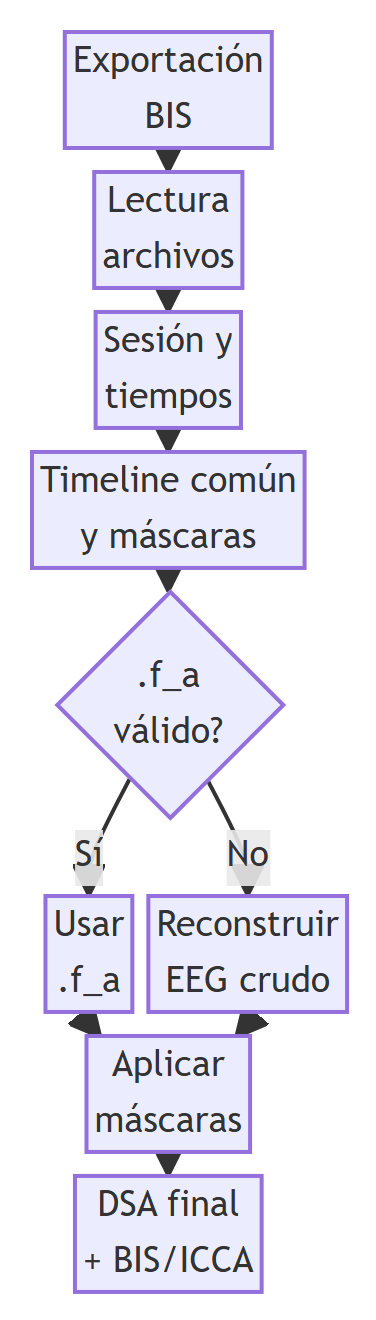
\includegraphics[width=3.4in,height=11.88in]{memoria_files/figure-latex/mermaid-figure-3.png}

}

\caption{\label{fig-flujo-dsa}Flujo general de obtención o
reconstrucción de la DSA. Fuente: elaboración propia.}

\end{figure}%

\subsubsection{Preparación común de los datos
BIS}\label{preparaciuxf3n-comuxfan-de-los-datos-bis}

El tratamiento de la DSA parte de una fase común de lectura,
comprobación y alineación temporal de los archivos BIS. Esta fase se
aplica tanto cuando se utiliza la matriz espectral original del archivo
\texttt{.f\_a} como cuando la DSA debe reconstruirse a partir de la
señal EEG cruda.

Los archivos exportados por el monitor no son perfectos y se puede
perder información (saltos temporales, registros duplicados) por razones
como movimientos del paciente, sudor, mala colocación de los sensores,
etc. Para evitar que esto interfiera en la visualización de la
información, antes de reconstruir o comparar matrices espectrales se
realiza una alineación temporal de los archivos: - se ordenan los
registros cronológicamente, - se unifica el formato de las marcas
temporales (DD/MM/AAAA HH:MM:SS), - en los archivos \texttt{.spa} y
\texttt{.f\_a} se eliminan aquellos segundos duplicados y se conserva la
última aparición de los mismos. En ellos también se detectan los huecos
temporales causados por pérdida de registros. - se detectan los posibles
segundos incompletos en el final del archivo de señal cruda.

Con esta información se construye una línea temporal común con
resolución de un segundo. Esta línea temporal se obtiene a partir del
intervalo compartido por las fuentes disponibles, evitando prolongar
artificialmente ningún archivo fuera de su cobertura real. Los datos del
\texttt{.spa}, la DSA original del \texttt{.f\_a} o la DSA reconstruida
se ajustan posteriormente a este intervalo.

Esta línea común permite alinear la DSA, las variables procesadas del
archivo \texttt{.spa} y, posteriormente, las variables clínicas
procedentes de ICCA. Los archivos se recortan o ajustan al intervalo de
la sesión BIS, pero los huecos detectados no se eliminan de forma
silenciosa: se conservan como instantes sin información válida para
poder identificarlos mediante máscaras.

Esta normalización temporal permite revisar qué ocurría en el ámbito
neurológico del paciente mientras se aporta su contexto clínico durante
un periodo de tiempo concreto.

\subsection{\texorpdfstring{Uso de la DSA original del archivo
\texttt{.f\_a}}{Uso de la DSA original del archivo .f\_a}}\label{uso-de-la-dsa-original-del-archivo-.f_a}

Cuando el archivo \texttt{.f\_a} está disponible y contiene información
válida, la aplicación permite utilizar la matriz espectral exportada por
el monitor como DSA original. En este caso no se realiza una
reconstrucción espectral desde la señal cruda, sino que se lee
directamente la matriz calculada por el dispositivo.

Como se detalla en los anexos, en registros unilaterales, el archivo
\texttt{.f\_a} contiene una columna temporal y una columna espectral. En
registros bilaterales, contiene una columna temporal y dos columnas
espectrales, correspondientes a los lados izquierdo y derecho. Cada fila
incluye los valores espectrales de 60 bins de frecuencia, desde 0,5
hasta 30 Hz con resolución de 0,5 Hz \citep{CovidienSerial2010}.

Los valores espectrales del \texttt{.f\_a} se leen como valores
numéricos codificados y se reescalan dividiéndolos entre 100 para
obtener los valores de la matriz en decibelios (\texttt{dB}).
Posteriormente, la matriz se ajusta a la línea temporal de la sesión.
Los segundos presentes en la timeline pero ausentes en la matriz se
mantienen como valores no disponibles, de forma que no se genera
continuidad artificial.

La DSA original se representa con una escala visual fija de 49 a 94 dB,
equivalente a la escala empleada en la visualización del monitor
\citep{CovidienBISVista, CovidienVISTABilateral}. Sobre esta matriz se
superponen las variables procesadas procedentes del \texttt{.spa}, como
SEF, MEF, BIS, EMG, SR y, en registros bilaterales, ASYM09.

\begin{figure}

\centering{

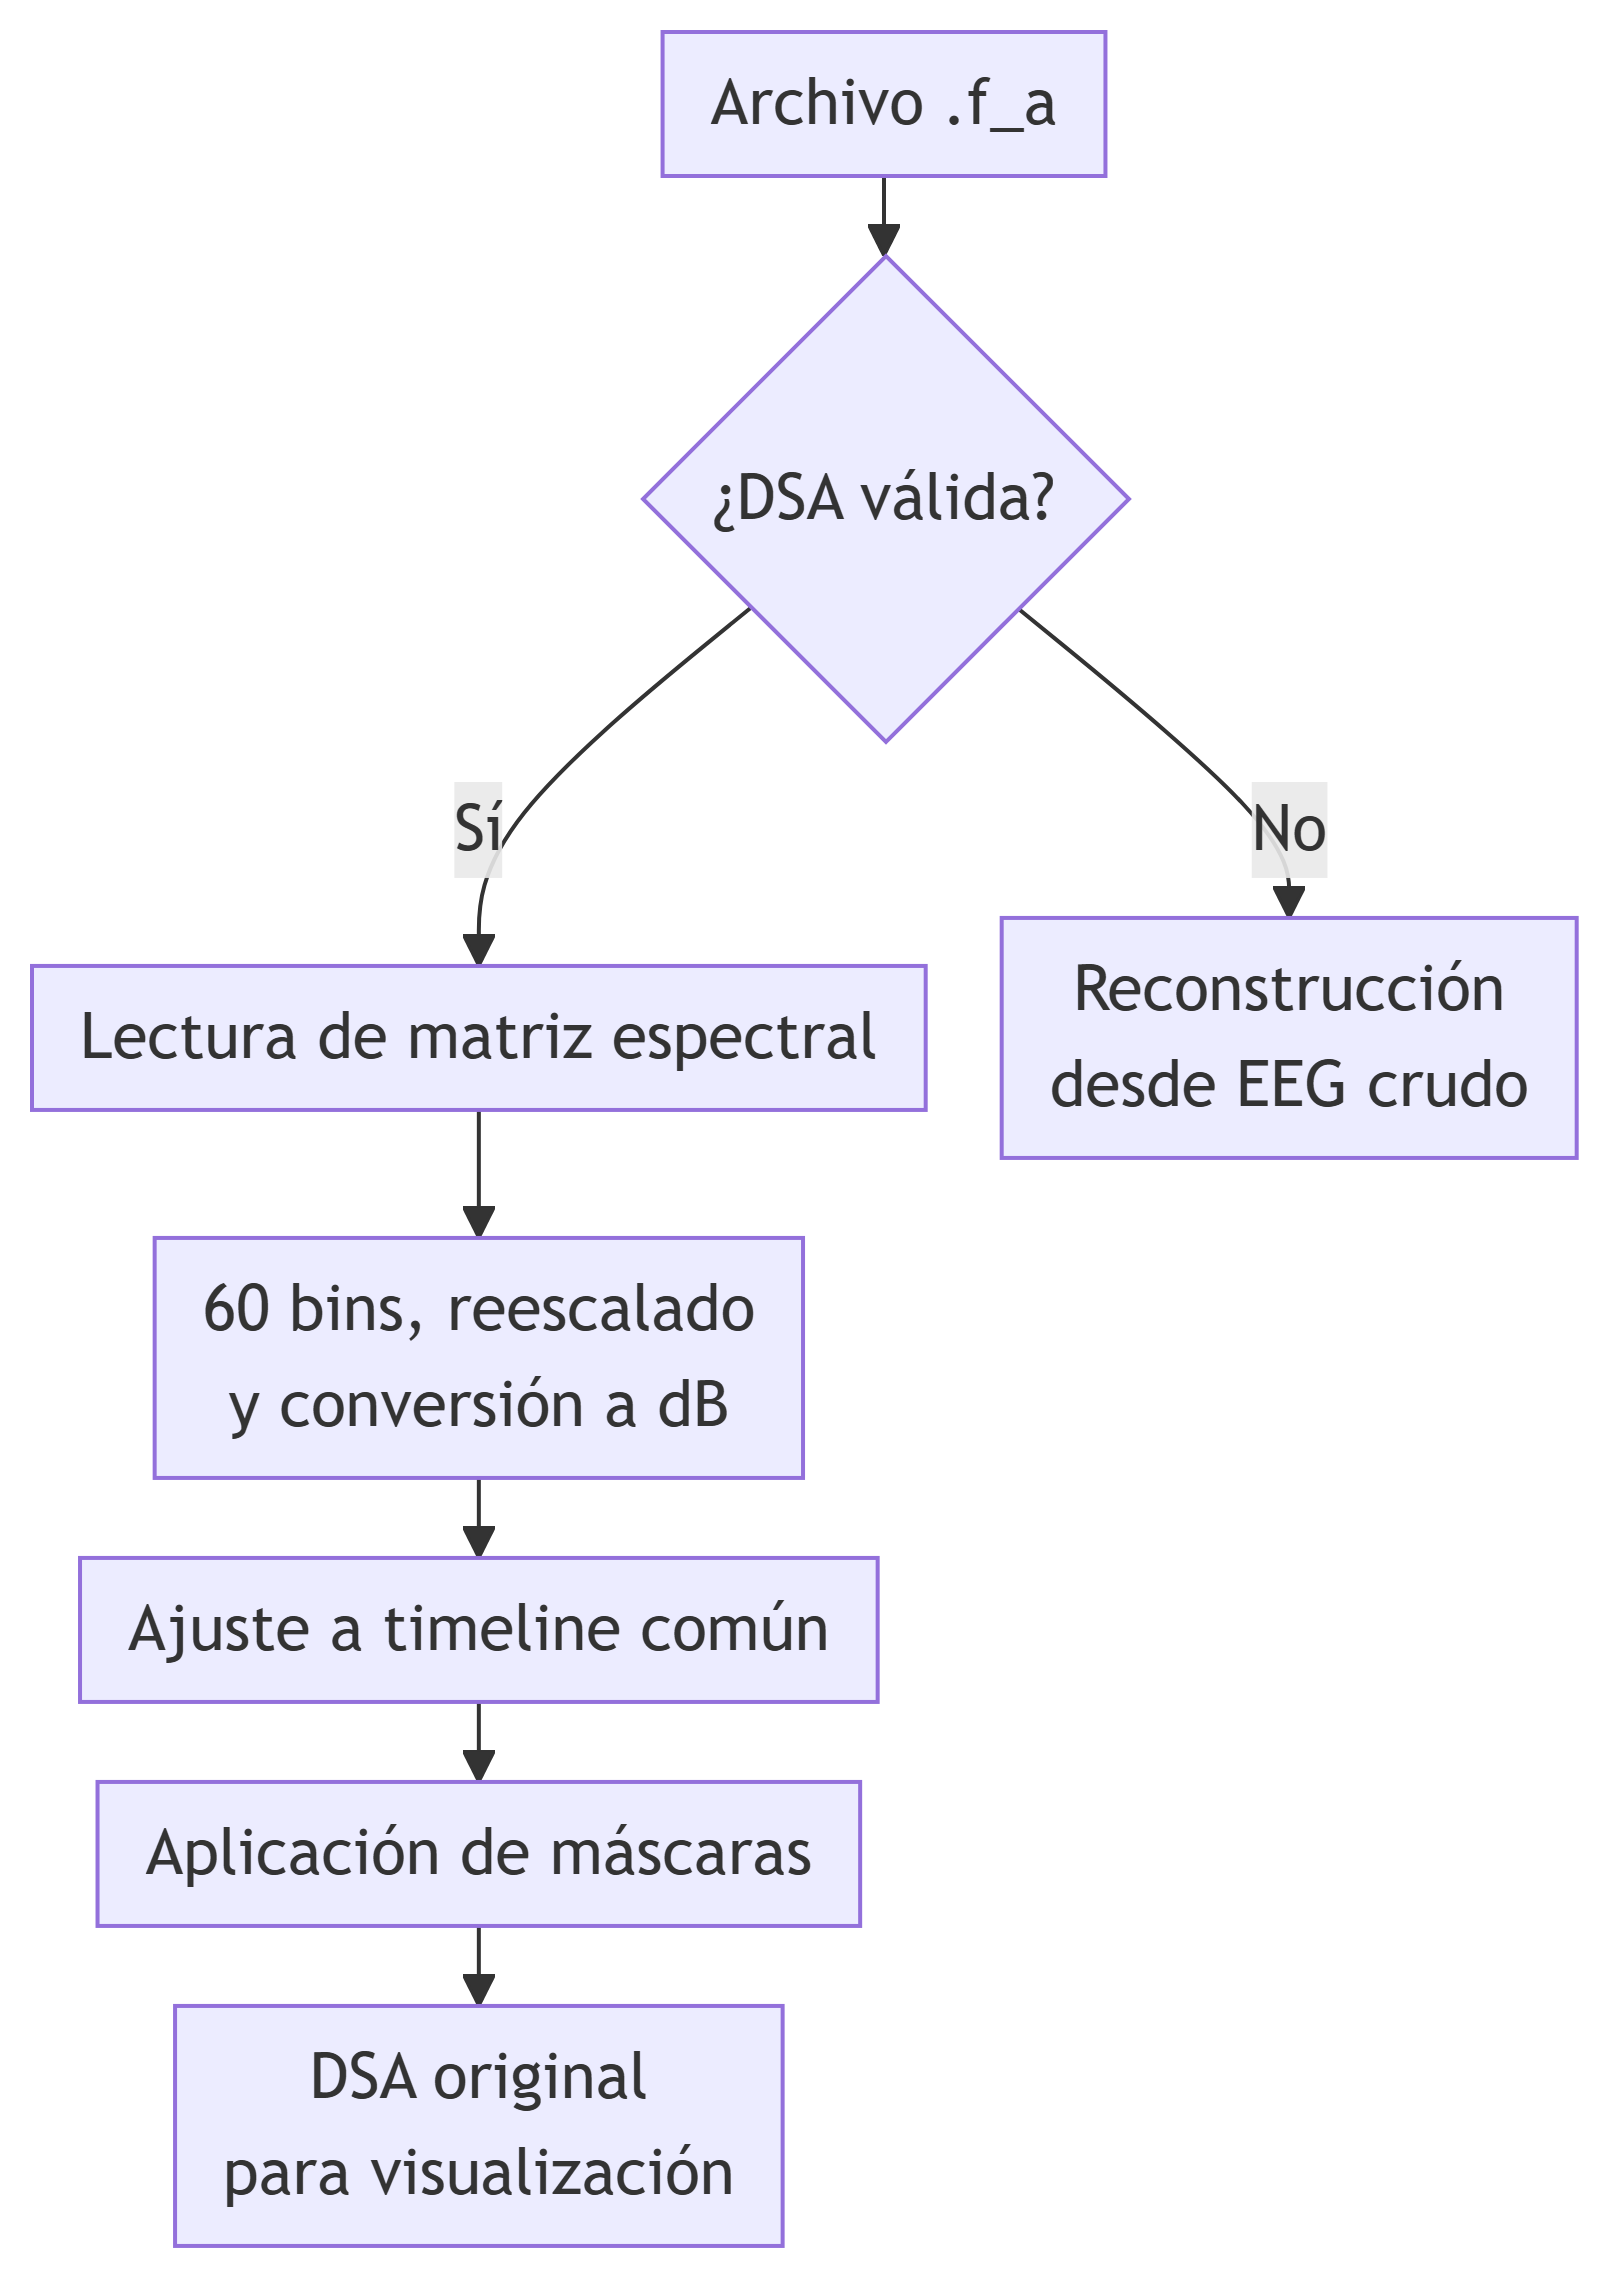
\includegraphics[width=4in,height=5.66in]{memoria_files/figure-latex/mermaid-figure-2.png}

}

\caption{\label{fig-flujo-fa}Flujo de uso de la matriz espectral
original del archivo \texttt{.f\_a}. Fuente: elaboración propia.}

\end{figure}%

\subsection{Máscaras de calidad}\label{muxe1scaras-de-calidad}

Para evitar que la visualización sugiera continuidad o fiabilidad en
tramos problemáticos, se genera una máscara de calidad sobre la timeline
común. Un segundo se considera no válido cuando se cumple alguno de los
siguientes criterios:

\begin{itemize}
\tightlist
\item
  \textbf{Pérdida de señal cruda.} Dentro de las 128 muestras que forman
  un segundo en un canal, si el 50 \% o más son exactamente cero, ese
  segundo se invalida por completo. Este criterio se basa en que, ante
  la pérdida de paquetes de EEG, el propio equipo rellena las muestras
  ausentes con ceros para mantener la continuidad temporal
  \citep{CovidienSerial2010}. Los ceros aislados y esporádicos, que no
  alcanzan ese 50 \%, no invalidan el segundo.
\item
  \textbf{Huecos temporales rellenados artificialmente.} Cuando la
  alineación temporal detecta un salto entre los archivos
  \texttt{.spa}/\texttt{.f\_a} (por ejemplo, si se dispone del segundo
  14 y del segundo 16 pero falta el 15), el segundo intermedio se añade
  de forma artificial para completar la timeline común. Al tratarse de
  un valor generado y no de un dato real, ese segundo también se
  invalida.
\item
  \textbf{Calidad de señal o potencia insuficiente}, según los criterios
  ya descritos en el Anexo F: \texttt{SQI10} inferior a 15 o
  \texttt{TOTPOW08} ausente o con valor centinela.
\item
  \textbf{Primer segundo del array reconstruido.} Al emplear una ventana
  de Welch de 2 segundos, existe sistemáticamente un desfase de un
  segundo entre el array del archivo \texttt{.f\_a} y el array de la DSA
  reconstruida; por este motivo, el primer segundo de la reconstrucción
  se invalida siempre, con independencia de la calidad de la señal.
\item
  \textbf{Propagación desde el EEG crudo.} Cuando un segundo del archivo
  crudo ha sido invalidado por el criterio de pérdida de señal,
  cualquier ventana de Welch que incorpore esas muestras no puede
  calcularse, ya que la estimación espectral no admite valores ausentes
  (NaN). En consecuencia, la invalidación de un segundo del EEG crudo se
  propaga a todas las ventanas espectrales que dependen de él.
\end{itemize}

La máscara se aplica al final de todo el procesamiento, tanto si la DSA
procede de la reconstrucción ---una vez aplicados el suavizado y el
desplazamiento temporal--- como si procede directamente del archivo
\texttt{.f\_a}. No obstante, los segundos inválidos están presentes como
valores ausentes (NaN) durante todos los pasos intermedios: no se
suavizan, no se filtran ni se incluyen en el cálculo de Welch como si
fuesen datos reales. Únicamente al final del proceso se representan en
blanco en la visualización.

En registros bilaterales, la máscara se calcula de forma independiente
para cada hemisferio. Las variables asociadas a cada lado, como SEF,
MEF, BIS, EMG y SR, se enmascaran siguiendo la máscara correspondiente a
su hemisferio. En el caso de \texttt{ASYM09}, el valor se considera no
válido cuando falta información válida en cualquiera de los dos
hemisferios.

La aplicación de esta máscara permite conservar la estructura temporal
del registro sin representar como válidos tramos en los que la
información disponible ---ya sea por pérdida de señal, huecos temporales
o límites del propio método de estimación--- no permite una
interpretación fiable.

\subsection{Reconstrucción desde EEG
crudo}\label{reconstrucciuxf3n-desde-eeg-crudo}

Cuando el archivo \texttt{.f\_a} no existe, está vacío o se desea
comparar la matriz exportada con una reconstrucción independiente, la
DSA se reconstruye a partir de la señal EEG cruda almacenada en
\texttt{.r2a} o \texttt{.r4a}. Esta reconstrucción incluye la conversión
de la señal cruda a microvoltios, el filtrado previo, la estimación
espectral mediante Welch y FFT, la conversión a decibelios, el
suavizado, el ajuste temporal y la aplicación de máscaras.

Dado que esta parte constituye el bloque metodológico más experimental
del trabajo, su desarrollo detallado se recoge en el Anexo G. En dicho
anexo se describen los parámetros empleados, las pruebas realizadas, el
suavizado, el desplazamiento temporal y la validación frente a la DSA
original cuando el archivo \texttt{.f\_a} está disponible.

\section{Integración temporal de los datos
ICCA}\label{integraciuxf3n-temporal-de-los-datos-icca}

Los datos clínicos procedentes de ICCA no se tratan como señales
continuas equivalentes al EEG, sino como información clínica contextual
asociada a la sesión BIS. Por ello, el tratamiento aplicado se centra en
su estructuración, recorte temporal y representación, respetando la
naturaleza de cada tipo de variable.

Para cada sesión BIS se genera, cuando existe información clínica
disponible, un archivo ICCA auxiliar recortado al intervalo temporal de
dicha sesión. De este modo, si un archivo ICCA contiene información de
varios días, pero la sesión BIS corresponde únicamente a un tramo
concreto, la aplicación conserva solo los datos clínicos relevantes para
ese intervalo. Los archivos originales no se modifican, sino que se
mantienen separados de los derivados generados durante el proceso.

El archivo ICCA auxiliar conserva la organización por hojas definida en
la plantilla clínica: información general, constantes vitales, análisis
clínicos y perfusiones. Esta separación permite representar cada grupo
de variables de acuerdo con su significado temporal. Las constantes
vitales se muestran como variables evolutivas; los análisis clínicos se
consideran mediciones puntuales; y las perfusiones se representan como
cambios de dosis activa en el tiempo.

En el caso de las constantes vitales, cuando es necesario para la
visualización, puede generarse una serie auxiliar a resolución de un
segundo. Estos valores intermedios se consideran sintéticos y se emplean
únicamente como apoyo visual, manteniendo siempre la trazabilidad de las
mediciones reales. Por tanto, no deben interpretarse como nuevas
mediciones clínicas ni utilizarse para validaciones clínicas o
correlaciones fuertes con las variables BIS.

Los análisis clínicos no se interpolan, sino que se muestran como
eventos puntuales asociados al instante en el que fueron registrados. En
el caso de variables sensibles al origen de la muestra, como la pO\(_2\)
o la pCO\(_2\), se aplica un criterio conservador: si no puede
determinarse con seguridad si la medición es arterial o venosa, el dato
se descarta para evitar errores de interpretación. Las perfusiones
tampoco se interpolan como valores acumulados, sino que se representan
como cambios documentados de dosis o velocidad, manteniendo su
comportamiento escalonado.

\section{Organización por paciente y
sesión}\label{organizaciuxf3n-por-paciente-y-sesiuxf3n}

La unidad básica de análisis del proyecto es la sesión BIS. Cada sesión
corresponde a un intervalo temporal concreto de monitorización
neurofisiológica y se asocia, cuando está disponible, a los datos
clínicos del mismo paciente procedentes de ICCA.

Para mantener la trazabilidad, los datos se organizan en carpetas por
paciente. Dentro de cada paciente se generan sesiones independientes,
formadas por una copia de la exportación BIS original y, en su caso, un
archivo ICCA auxiliar recortado al intervalo temporal correspondiente.
Esta organización permite trabajar con sesiones concretas sin modificar
los archivos originales.

Durante este proceso, la aplicación genera archivos de metadatos en
formato JSON, como \texttt{paciente.json} y \texttt{sesion.json}. Estos
archivos actúan como manifiestos de procedencia, ya que registran las
fuentes originales utilizadas, el tipo de monitorización BIS, los
intervalos temporales detectados y los archivos auxiliares generados.

\section{Visualización conjunta
BIS-DSA-ICCA}\label{visualizaciuxf3n-conjunta-bis-dsa-icca}

La visualización conjunta se desarrolló mediante Dash y Plotly. La
interfaz permite seleccionar un paciente, escoger una sesión BIS y
representar de forma integrada la información neurofisiológica y clínica
asociada al mismo intervalo temporal.

En la vista principal se muestra la DSA junto con las variables
procesadas del monitor BIS, como el índice BIS, SEF, MEF y, en registros
bilaterales, ASYM. También se incorporan variables de calidad o
contexto, como EMG y SR, cuando están disponibles.

Las variables clínicas procedentes de ICCA se incorporan sobre la misma
referencia temporal que la sesión BIS, pero sin transformar todas las
variables en una señal homogénea. Las constantes vitales se representan
como gráficas temporales, los análisis clínicos como mediciones
puntuales y las perfusiones como líneas escalonadas. Esta estrategia
permite revisar la evolución neurofisiológica junto con el contexto
clínico del paciente, preservando el significado temporal de cada tipo
de dato.

La interfaz permite seleccionar tramos horarios, modificar la duración
de la ventana visible y desplazarse por el registro. De esta forma, el
usuario puede revisar periodos concretos de interés y estudiar la
relación temporal entre los cambios observados en la DSA, las variables
BIS y la información clínica disponible.

\section{Metodología de Ingeniería del
Software}\label{metodologuxeda-de-ingenieruxeda-del-software}

\subsection{Estrategia de desarrollo}\label{estrategia-de-desarrollo}

El desarrollo se llevó a cabo de forma incremental, partiendo de
prototipos exploratorios en notebooks. En una primera fase se estudió la
estructura de los archivos BIS y se implementaron funciones de lectura,
decodificación y representación. Posteriormente, estas funciones se
separaron en módulos reutilizables y se integraron en aplicaciones
interactivas.

El proyecto evolucionó mediante ciclos de prueba y ajuste. Cada
iteración incorporó comprobaciones con registros reales unilaterales y
bilaterales, revisión visual de las salidas y validación cuantitativa
cuando existía una DSA exportada por el monitor. Esta estrategia
permitió avanzar desde pruebas aisladas de reconstrucción hacia una
herramienta integrada de análisis retrospectivo.

\subsection{Trazabilidad y
reproducibilidad}\label{trazabilidad-y-reproducibilidad}

La organización de los datos por paciente y sesión, descrita
anteriormente, ya aporta una primera capa de trazabilidad mediante la
separación entre archivos originales y derivados y los manifiestos
\texttt{paciente.json} y \texttt{sesion.json}. A nivel de desarrollo,
esta separación se completa con la posibilidad de regenerar los archivos
derivados a partir de las fuentes iniciales y de los parámetros
definidos en el procesamiento, sin necesidad de repetir manualmente cada
paso. Esto permite comparar configuraciones distintas de reconstrucción
o enmascarado y mantener siempre una relación clara entre cada resultado
mostrado y los archivos de entrada utilizados.

\subsection{Entorno de ejecución y máquinas
virtuales}\label{entorno-de-ejecuciuxf3n-y-muxe1quinas-virtuales}

La aplicación se ha preparado para poder ejecutarse en un entorno
controlado mediante máquinas virtuales, con el objetivo de aproximar su
funcionamiento a un posible despliegue dentro de una intranet
hospitalaria.

La arquitectura propuesta separa la ejecución de la aplicación y el
almacenamiento de los datos. Para ello, se plantea una máquina virtual
destinada a ejecutar la aplicación Dash y otra máquina virtual destinada
a actuar como repositorio común de pacientes.

La aplicación trabaja siempre sobre una ruta fija de pacientes, evitando
que el usuario tenga que seleccionar manualmente la carpeta de trabajo.
Los datos no se almacenan en una base de datos relacional, sino mediante
una estructura organizada de carpetas y archivos, acorde con el origen
de los registros utilizados en el proyecto.

Esta configuración permite simular un escenario en el que varios
usuarios acceden a una misma herramienta y consultan una ubicación común
de pacientes. La configuración técnica detallada de las máquinas
virtuales, la unidad compartida y el protocolo Samba/SMB se recoge en el
Anexo E (Manual del programador).

%% ── Capítulo 5: Resultados ──────────────────────────────────
\capitulo{5}{Resultados}

\section{Resumen de resultados}\label{resumen-de-resultados}

En este capítulo se presentan los principales resultados obtenidos tras
el desarrollo de la prueba de concepto. La exposición se organiza de
acuerdo con los objetivos específicos definidos previamente:
organización de datos BIS e ICCA, recuperación y reconstrucción de la
DSA, integración temporal de variables procesadas y clínicas, y
desarrollo del visualizador interactivo.

Como resultado global, se ha obtenido un flujo de trabajo que permite
organizar registros BIS e información clínica procedente de ICCA por
paciente y sesión, generar archivos auxiliares asociados a cada
intervalo de monitorización y visualizar de forma conjunta la matriz de
densidad espectral, las variables procesadas del monitor BIS y variables
clínicas relevantes para el análisis retrospectivo en UCI.

Los resultados experimentales detallados de la reconstrucción de la DSA,
incluyendo la comparación entre métodos espectrales, desplazamientos
temporales y métricas cuantitativas, se recogen en el Anexo G. El
detalle paso a paso de cómo se maneja cada interfaz (pantallas de
selección, creación y edición) se documenta en el Anexo D (Manual de
usuario); en este capítulo se muestran únicamente las capturas
necesarias para entender los resultados obtenidos.

\section{Organización de los datos BIS e
ICCA}\label{organizaciuxf3n-de-los-datos-bis-e-icca}

Uno de los resultados obtenidos fue la creación de una aplicación de
organización de datos que permite agrupar las exportaciones BIS y los
archivos clínicos procedentes de ICCA por paciente y sesión. Esta
herramienta, accesible desde el portal común a las tres aplicaciones
(Figura~\ref{fig-portal}), actúa como punto de entrada al flujo de
trabajo desarrollado, preparando los datos antes de su visualización
conjunta.

\begin{figure}

\centering{

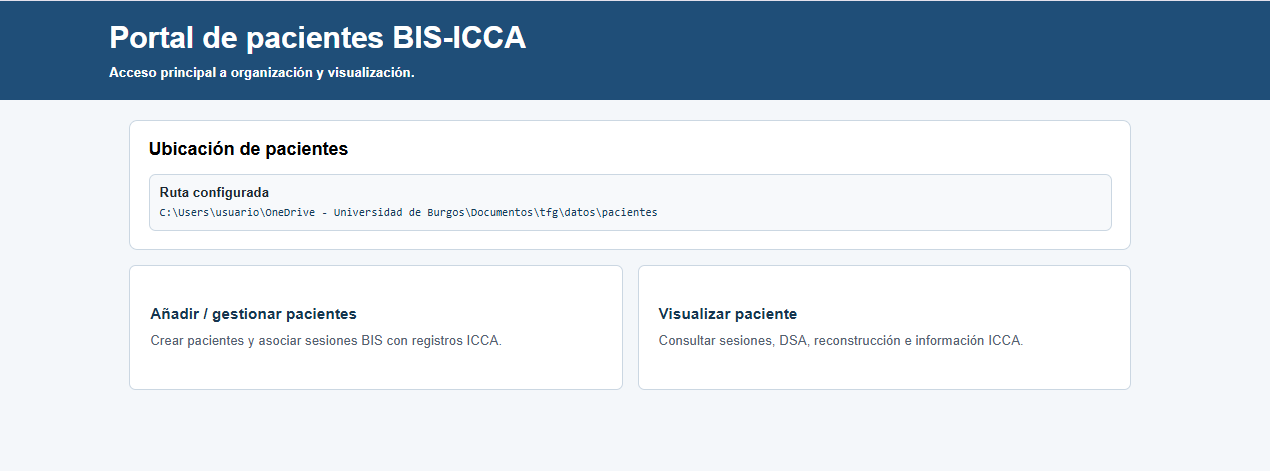
\includegraphics[width=0.9\linewidth,height=\textheight,keepaspectratio]{img/capturas_portal/captura_menu_portal.png}

}

\caption{\label{fig-portal}Portal de entrada a las aplicaciones
desarrolladas (organizador y visualizador). Fuente: elaboración propia.}

\end{figure}%

La aplicación permite seleccionar los archivos ICCA disponibles y una o
varias carpetas correspondientes a sesiones BIS, analiza los intervalos
temporales de cada fuente y, tras la revisión y confirmación del
usuario, crea una nueva carpeta de paciente organizada por sesiones, tal
y como se muestra en la Figura~\ref{fig-organizador-contenido-pac} (el
manejo detallado del resto de pantallas del organizador se recoge en el
Anexo D). El resultado de este proceso es una organización jerárquica en
la que cada paciente contiene una o varias sesiones BIS, cada una con la
exportación BIS original y, cuando existe información clínica
compatible, un archivo ICCA auxiliar recortado al intervalo
correspondiente.

\begin{figure}

\centering{

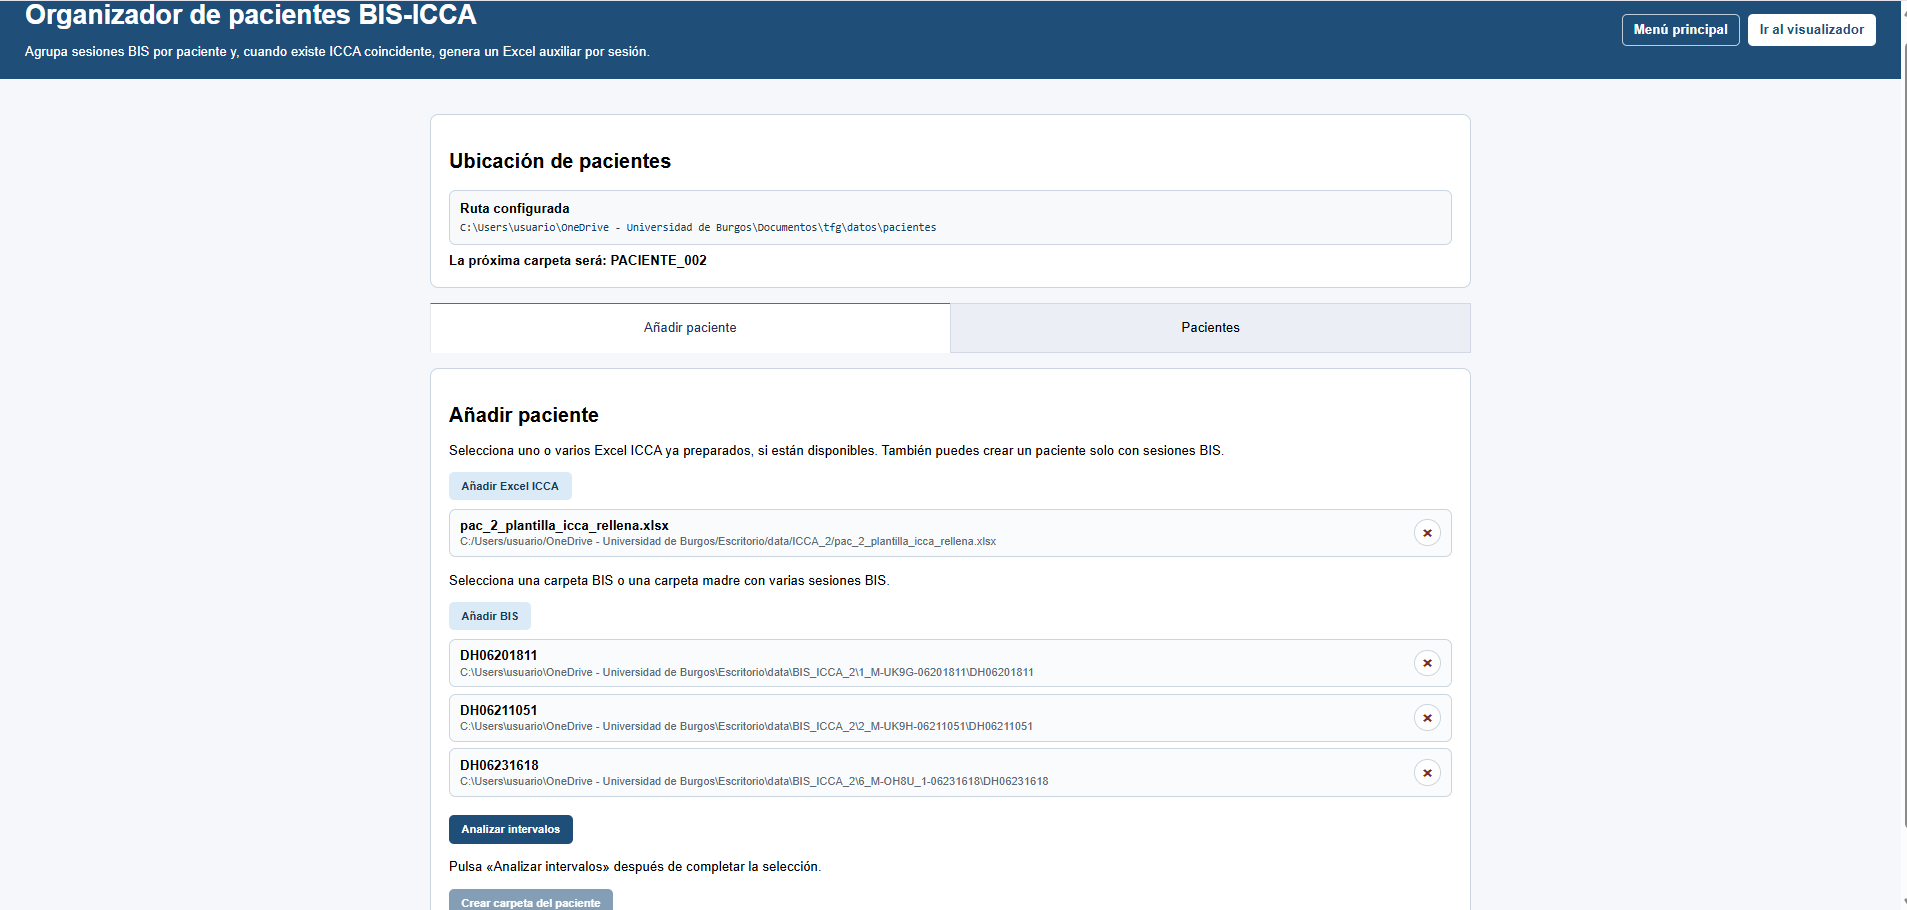
\includegraphics[width=0.9\linewidth,height=\textheight,keepaspectratio]{img/capturas_app_organizador/cap_crear_paciente.png}

}

\caption{\label{fig-organizador-contenido-pac}Creación de un nuevo
paciente a partir de archivos BIS e ICCA. Fuente: elaboración propia.}

\end{figure}%

\section{Recuperación y reconstrucción de la
DSA}\label{recuperaciuxf3n-y-reconstrucciuxf3n-de-la-dsa}

La aplicación de visualización permite consultar las sesiones
previamente organizadas, cargando la información neurofisiológica y
clínica correspondiente al intervalo de la sesión seleccionada (el
manejo de las pantallas de selección de paciente y sesión se documenta
en el Anexo D).

En relación con la matriz de densidad espectral, se consiguió
implementar un doble flujo de trabajo. Cuando el archivo \texttt{.f\_a}
está disponible y contiene información válida, la aplicación permite
utilizar directamente la matriz espectral exportada por el monitor, tal
y como se muestra en la Figura~\ref{fig-visualizador-dsa-fa-unilat}. En
cambio, cuando este archivo no existe o está vacío, la DSA se
reconstruye a partir de la señal EEG cruda almacenada en \texttt{.r2a} o
\texttt{.r4a}, según se observa en la
Figura~\ref{fig-visualizador-dsa-rec-unilat}.

\begin{figure}

\centering{

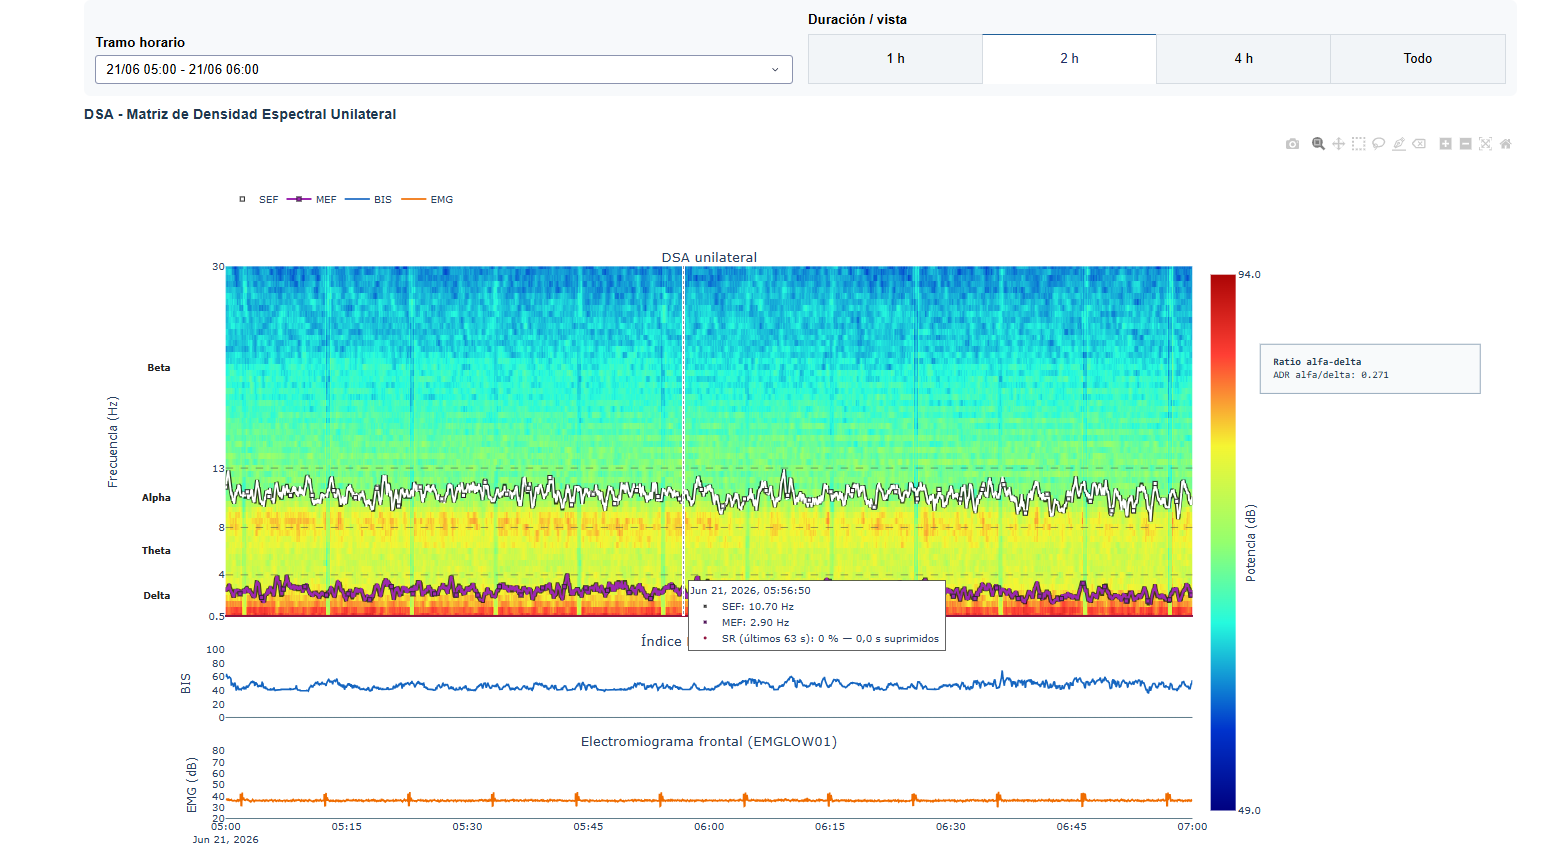
\includegraphics[width=0.9\linewidth,height=\textheight,keepaspectratio]{img/capturas_app_visualizador/visual_DSA_reconstruida_unilateral.png}

}

\caption{\label{fig-visualizador-dsa-rec-unilat}Visualización de una DSA
unilateral reconstruida a partir del EEG crudo. Fuente: elaboración
propia.}

\end{figure}%

\begin{figure}

\centering{

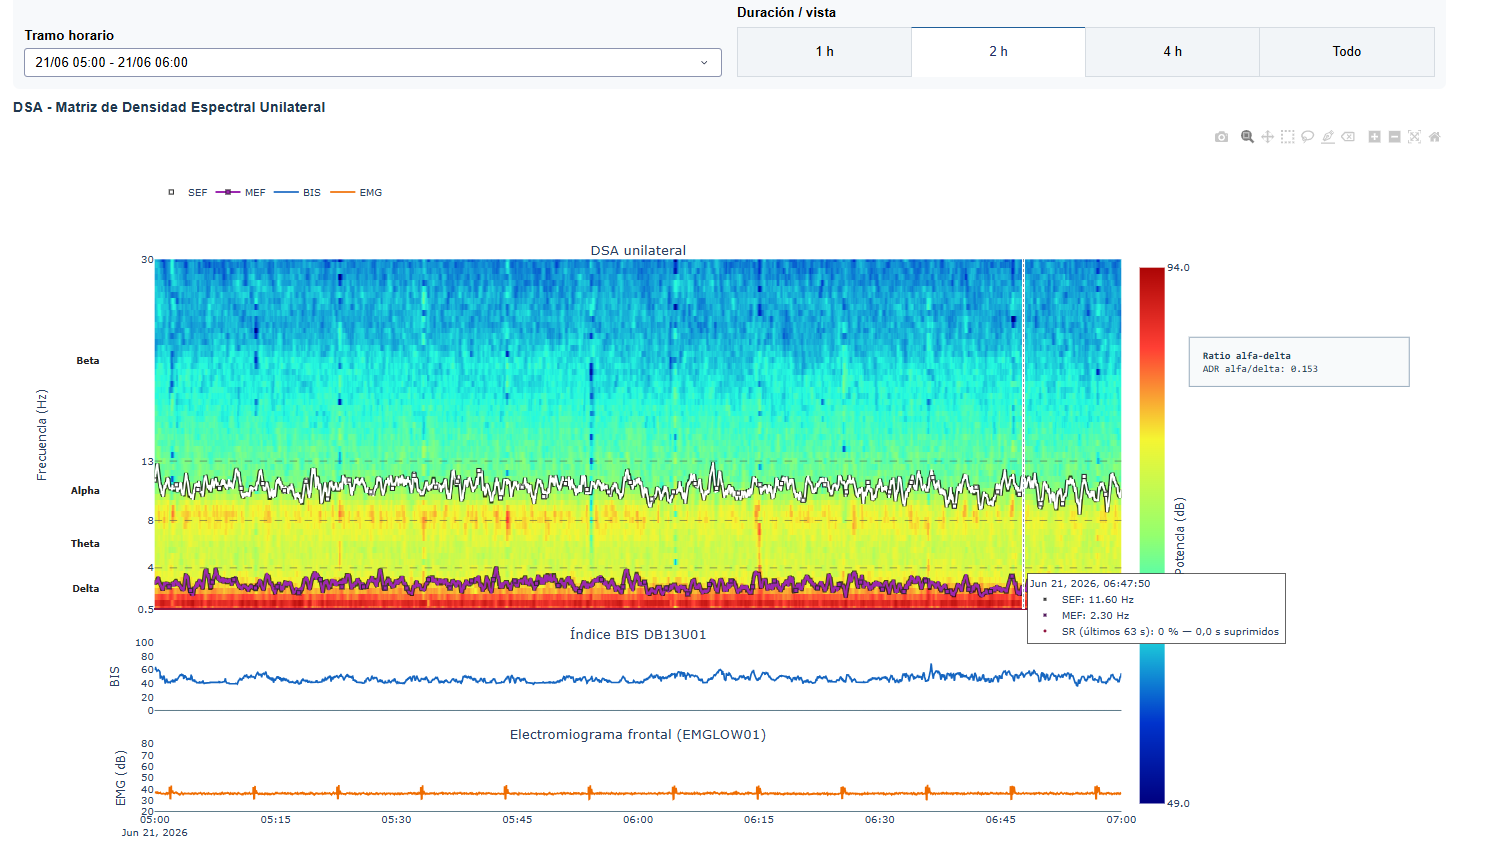
\includegraphics[width=0.9\linewidth,height=\textheight,keepaspectratio]{img/capturas_app_visualizador/visual_DSA_fa_unilateral.png}

}

\caption{\label{fig-visualizador-dsa-fa-unilat}Visualización de una DSA
unilateral obtenida directamente desde el archivo espectral
\texttt{.f\_a}. Fuente: elaboración propia.}

\end{figure}%

Estas dos figuras muestran ambos escenarios en un registro unilateral.
Esta doble posibilidad resulta importante porque no todas las sesiones
disponibles contienen un archivo \texttt{.f\_a} válido.

También se comprobó el funcionamiento del sistema en un registro
procedente de BIS VISTA sin información clínica ICCA asociada y sin
matriz \texttt{.f\_a} válida: en concreto, un autorregistro realizado
por la propia alumna para explorar el formato real de los archivos BIS
antes de disponer de la aprobación del Comité de Bioética (ver
Discusión), y que por tanto no tiene un archivo ICCA con el que
relacionarse. Este caso resulta útil precisamente porque no deja
alternativa: al no existir ni \texttt{.f\_a} válido ni ICCA asociado, la
única vía posible es forzar la reconstrucción completa de la DSA desde
la señal cruda, tal y como se refleja en la selección de la sesión
(Figura~\ref{fig-visualizador-seleccionar-pac-vista}).

\begin{figure}

\centering{

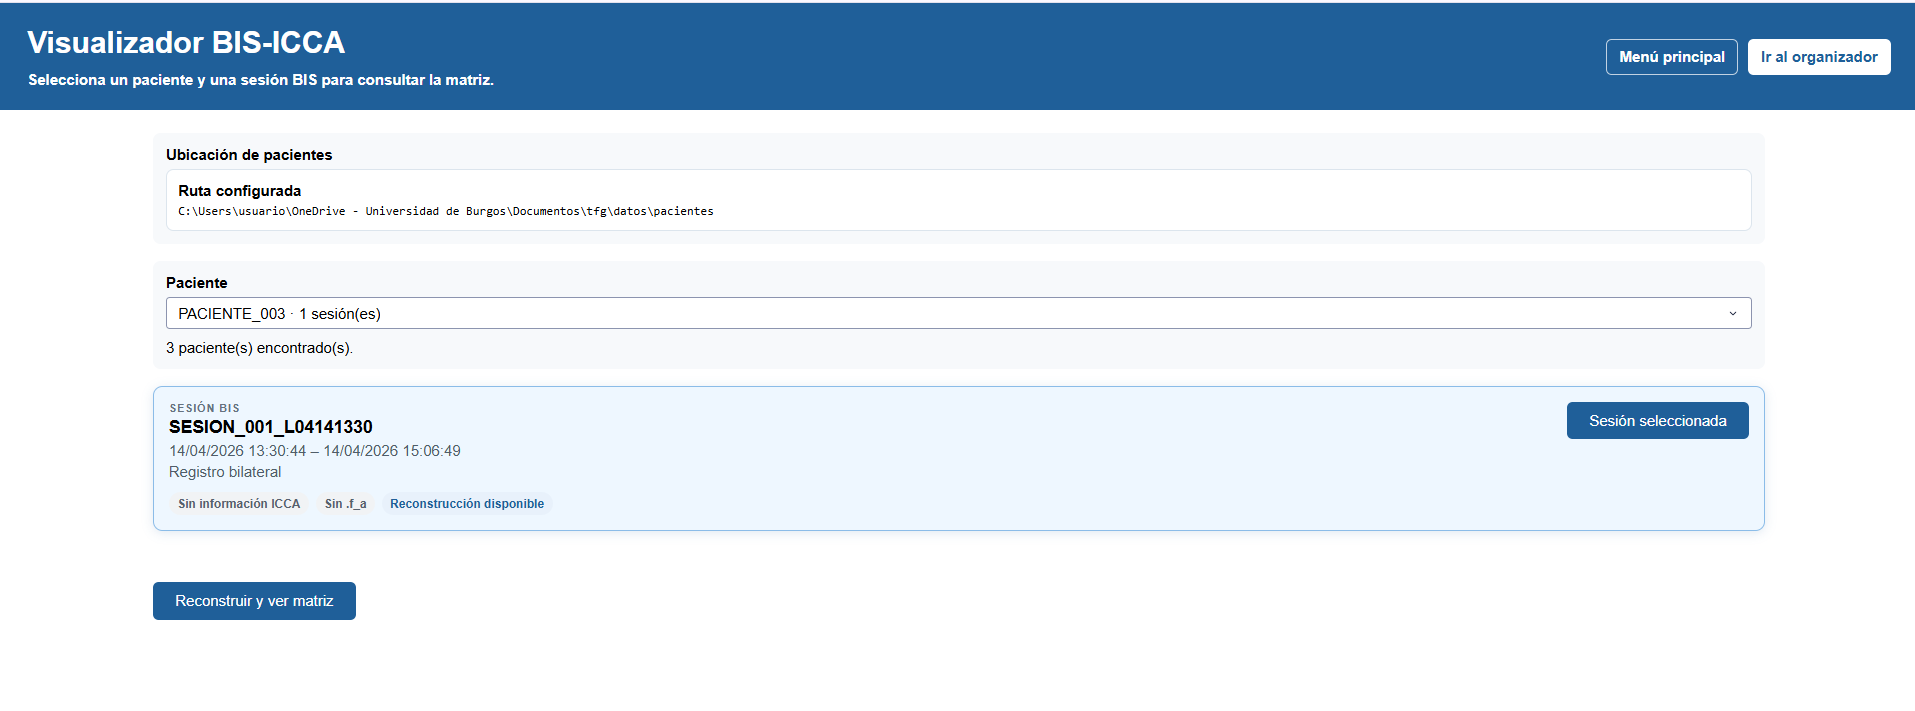
\includegraphics[width=0.9\linewidth,height=\textheight,keepaspectratio]{img/capturas_app_visualizador/visual_sinICCA_sinFA.png}

}

\caption{\label{fig-visualizador-seleccionar-pac-vista}Selección de una
sesión BIS VISTA (autorregistro) sin ICCA asociado y sin archivo
\texttt{.f\_a} válido. Fuente: elaboración propia.}

\end{figure}%

El visualizador carga igualmente la sesión BIS y fuerza la
reconstrucción de la DSA a partir de la señal cruda, incluyendo la
reconstrucción bilateral cuando el registro dispone de los dos
hemisferios, tal y como se muestra en la
Figura~\ref{fig-visualizador-dsa-rec-bilat}.

\begin{figure}

\centering{

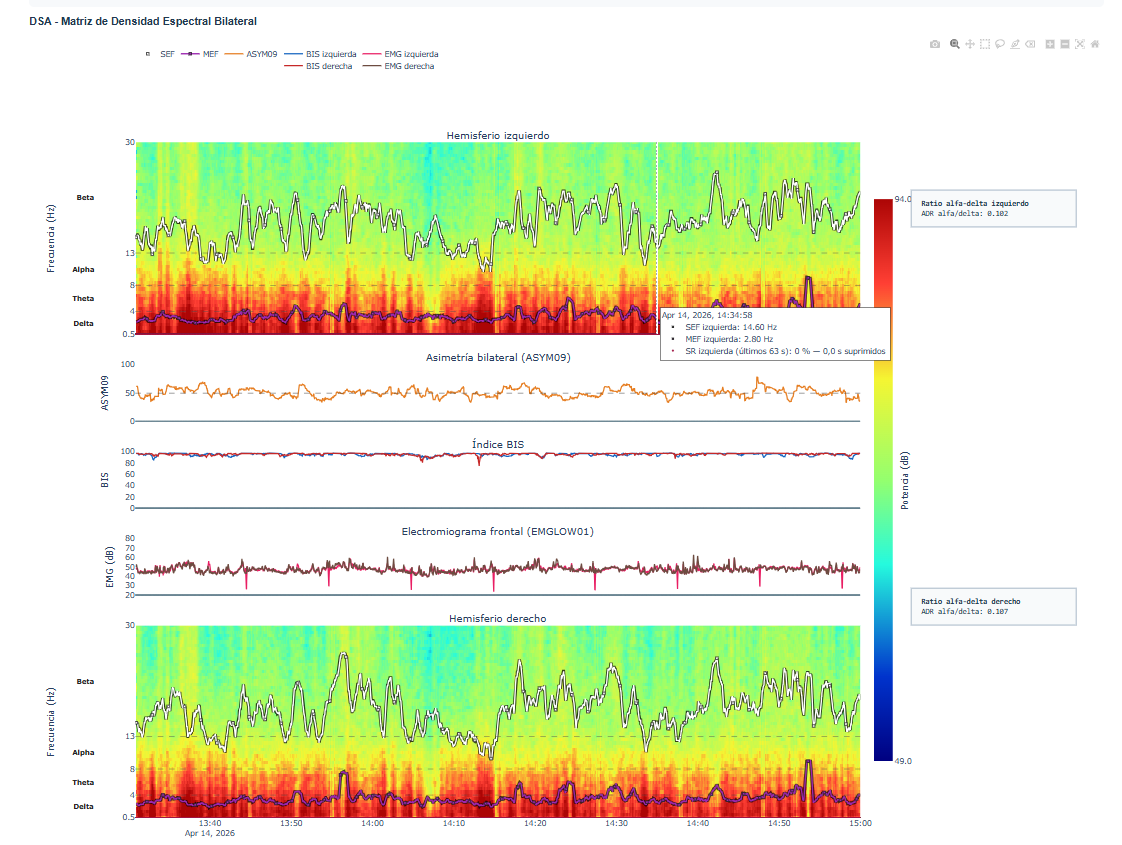
\includegraphics[width=0.9\linewidth,height=\textheight,keepaspectratio]{img/capturas_app_visualizador/visual_VISTA_bilat.png}

}

\caption{\label{fig-visualizador-dsa-rec-bilat}Reconstrucción bilateral
de la DSA en un registro BIS VISTA sin archivo \texttt{.f\_a} válido y
sin información ICCA asociada. Fuente: elaboración propia.}

\end{figure}%

El sistema distingue automáticamente entre registros unilaterales y
bilaterales a partir del archivo de EEG crudo disponible. En los
registros unilaterales se genera una única matriz DSA, mientras que en
los registros bilaterales se obtienen dos matrices independientes,
correspondientes a los hemisferios izquierdo y derecho.

\section{Integración temporal de variables
BIS}\label{integraciuxf3n-temporal-de-variables-bis}

Además de la DSA, se consiguió representar las principales variables
procesadas del monitor BIS dentro de una misma línea temporal. Entre
ellas se incluyen el índice BIS, la frecuencia espectral de borde, la
frecuencia mediana y, en los registros bilaterales, la asimetría entre
hemisferios (visibles ya en las capturas anteriores, de la
Figura~\ref{fig-visualizador-dsa-rec-unilat} a la
Figura~\ref{fig-visualizador-dsa-rec-bilat}).

La aplicación incluye criterios de calidad para evitar la representación
de intervalos no fiables. Los tramos con baja calidad de señal, ausencia
de información espectral o discontinuidades se muestran como periodos no
válidos. De este modo, la visualización evita presentar como
fisiológicamente interpretables aquellos instantes en los que la señal o
la matriz espectral no contienen información suficiente.

\section{Integración de variables clínicas
ICCA}\label{integraciuxf3n-de-variables-cluxednicas-icca}

Las variables clínicas procedentes de ICCA se incorporaron al flujo de
visualización mediante plantillas estructuradas. La información se
organizó en datos generales, constantes vitales, resultados analíticos y
perfusiones, representando cada tipo de variable de acuerdo con su
naturaleza temporal.

Las constantes vitales se trataron como series temporales asociadas al
intervalo de la sesión BIS, tal y como se muestra en la
Figura~\ref{fig-visualizador-cte-icca}.

\begin{figure}

\centering{

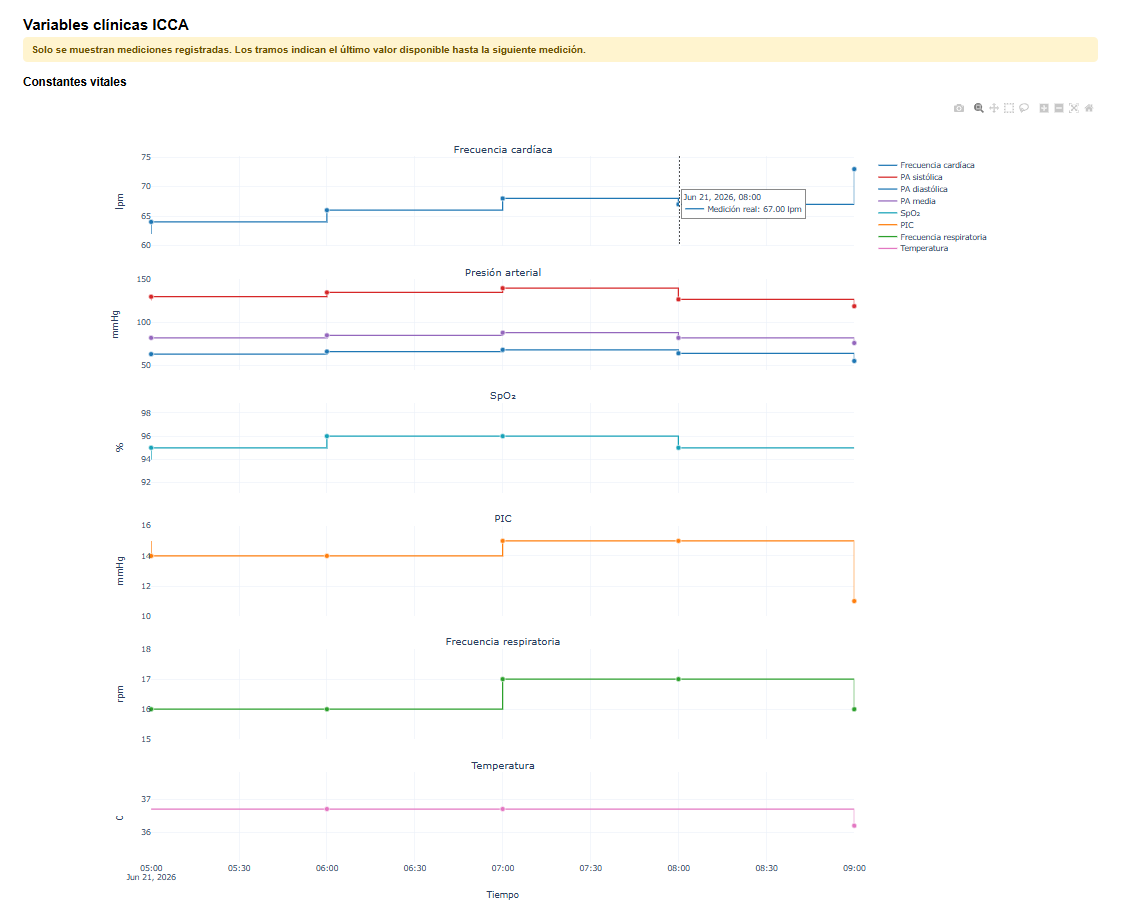
\includegraphics[width=0.9\linewidth,height=\textheight,keepaspectratio]{img/capturas_app_visualizador/visual_variables_clinicas.png}

}

\caption{\label{fig-visualizador-cte-icca}Representación de constantes
clínicas procedentes de ICCA, como series temporales asociadas al
intervalo de la sesión. Fuente: elaboración propia.}

\end{figure}%

Los análisis clínicos se representaron como mediciones puntuales,
conservando su instante de registro
(Figura~\ref{fig-visualizador-analisis-icca}).

\begin{figure}

\centering{

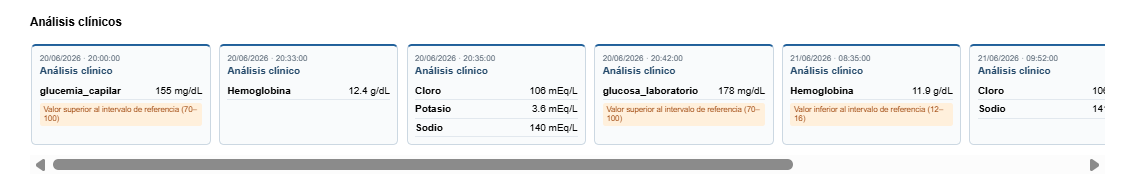
\includegraphics[width=0.9\linewidth,height=\textheight,keepaspectratio]{img/capturas_app_visualizador/visual_tarjetas_analisis.png}

}

\caption{\label{fig-visualizador-analisis-icca}Visualización de
resultados analíticos asociados a la sesión BIS, como mediciones
puntuales. Fuente: elaboración propia.}

\end{figure}%

Las perfusiones se incorporaron como cambios de dosis activa a lo largo
del tiempo, lo que permite estudiar su relación temporal con la
evolución del BIS y de la DSA
(Figura~\ref{fig-visualizador-perfusiones-icca}).

\begin{figure}

\centering{

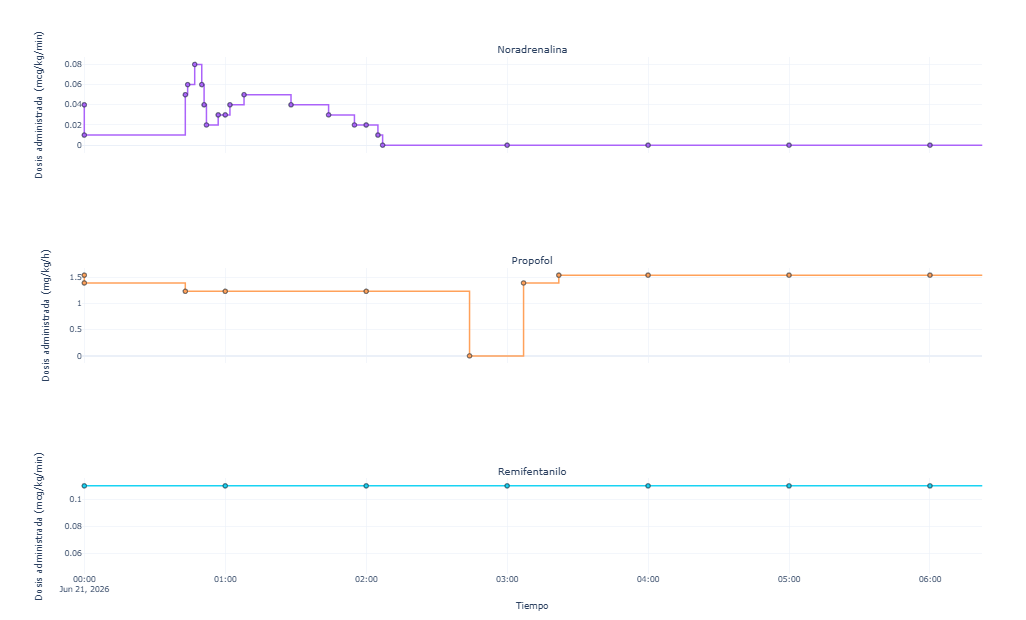
\includegraphics[width=0.9\linewidth,height=\textheight,keepaspectratio]{img/capturas_app_visualizador/visual_perfusiones_2.png}

}

\caption{\label{fig-visualizador-perfusiones-icca}Representación de
perfusiones y tratamientos administrados durante el intervalo analizado,
como cambios de dosis activa. Fuente: elaboración propia.}

\end{figure}%

La integración de estas variables permite contextualizar la evolución
neurofisiológica del paciente con información clínica relevante, como
cambios hemodinámicos, alteraciones analíticas o administración de
sedantes, analgésicos, relajantes neuromusculares y fármacos
vasoactivos.

\section{Visualizador interactivo
desarrollado}\label{visualizador-interactivo-desarrollado}

El resultado final de esta parte del proyecto es un visualizador
interactivo que permite explorar registros BIS unilaterales y
bilaterales junto con la información clínica disponible, seleccionar
paciente y sesión, modificar la ventana temporal visible y revisar
periodos concretos del registro (Anexo D). En registros bilaterales, el
visualizador muestra de forma diferenciada la información
correspondiente a ambos hemisferios, incluyendo las matrices DSA
izquierda y derecha, las curvas BIS asociadas y la asimetría bilateral,
como ya se ha mostrado en la
Figura~\ref{fig-visualizador-dsa-rec-bilat}.

\section{Generación de informe en
PDF}\label{generaciuxf3n-de-informe-en-pdf}

Como resultado complementario del visualizador, se incorporó la
posibilidad de generar un informe en formato PDF asociado a una sesión
BIS concreta. El documento se organiza en tres bloques: una portada con
los datos identificativos de la sesión, una página con la representación
completa de la DSA junto con las variables procesadas del monitor, y un
resumen textual de la información clínica ICCA del intervalo, cuando
está disponible.

La portada recoge los datos identificativos de la sesión (paciente,
sesión BIS, tipo de registro, origen de la DSA, intervalo temporal
analizado y disponibilidad de información ICCA), tal y como se muestra
en la Figura~\ref{fig-informe-pdf}.

\begin{figure}

\centering{

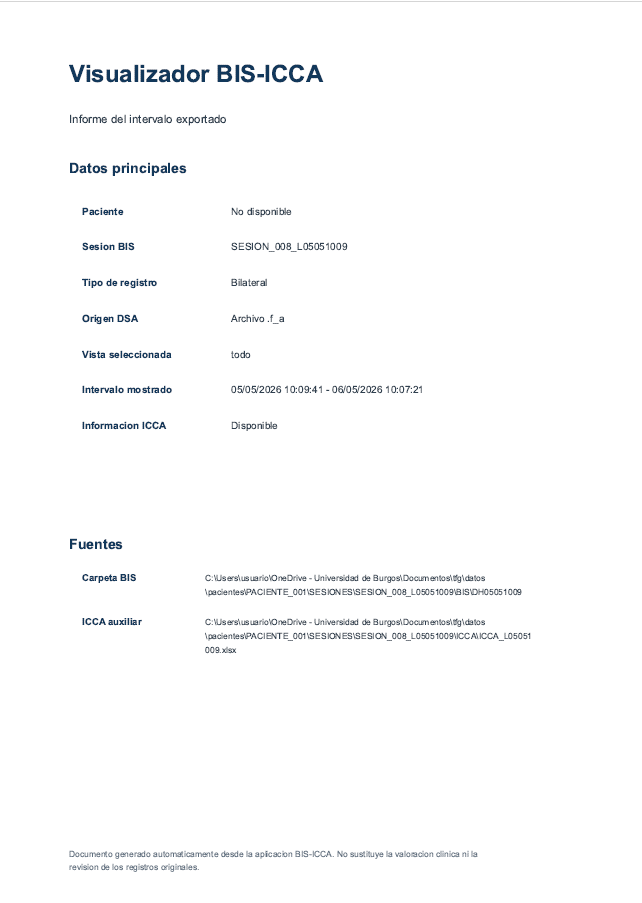
\includegraphics[width=0.9\linewidth,height=\textheight,keepaspectratio]{img/capturas_app_visualizador/visual_informe_pdf.png}

}

\caption{\label{fig-informe-pdf}Portada del informe PDF, con los datos
identificativos de la sesión. Fuente: elaboración propia.}

\end{figure}%

A continuación, el informe incluye la representación completa de la DSA
y las variables procesadas del monitor correspondientes al intervalo
mostrado (Figura~\ref{fig-informe-dsa-pdf}), y finaliza con un resumen
textual de la información clínica ICCA disponible para ese mismo
intervalo (Figura~\ref{fig-informe-analisis-pdf}).

\begin{figure}

\centering{

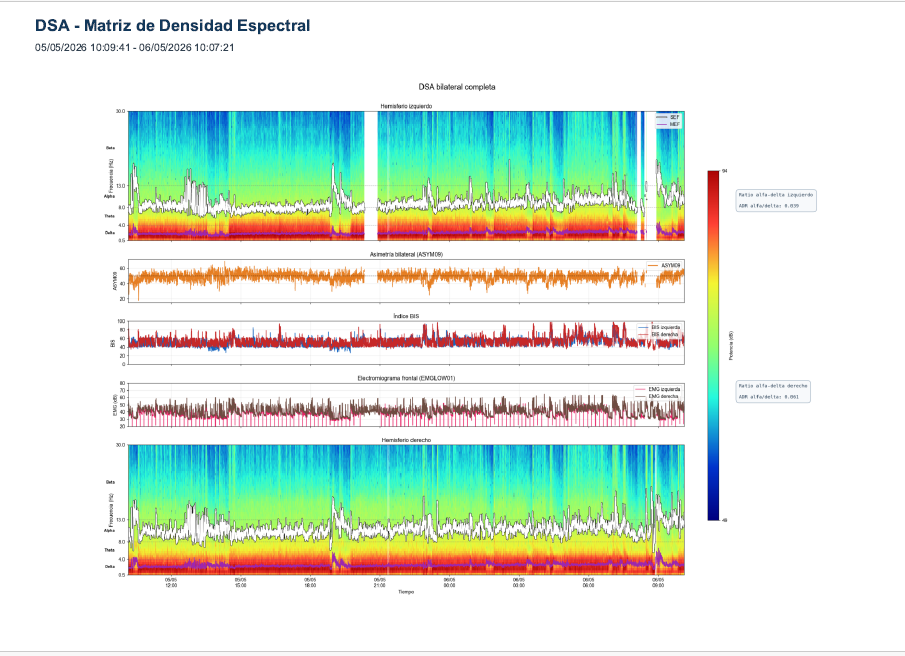
\includegraphics[width=0.9\linewidth,height=\textheight,keepaspectratio]{img/capturas_app_visualizador/visual_informe_2_pdf.png}

}

\caption{\label{fig-informe-dsa-pdf}Página de la DSA y las variables
procesadas del monitor en el informe PDF. Fuente: elaboración propia.}

\end{figure}%

\begin{figure}

\centering{

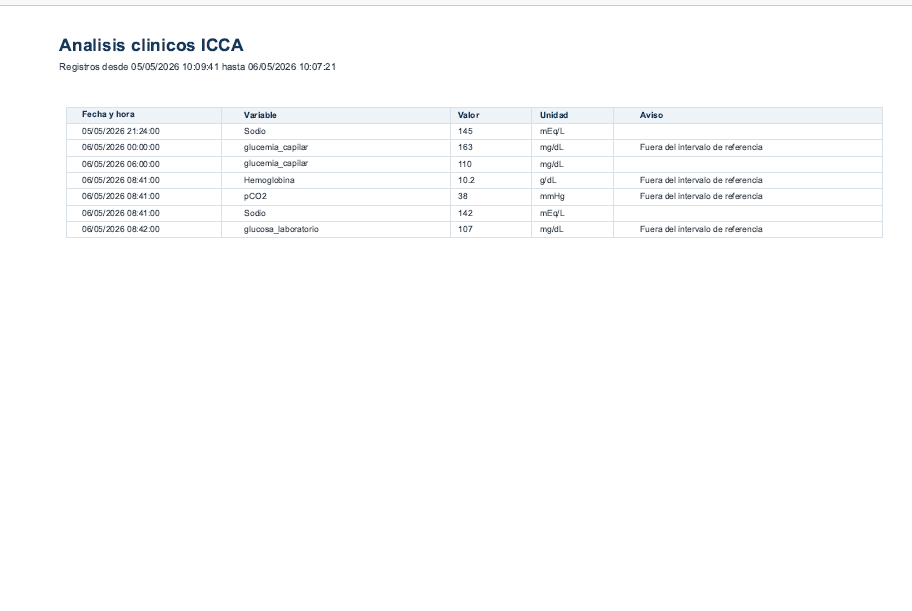
\includegraphics[width=0.9\linewidth,height=\textheight,keepaspectratio]{img/capturas_app_visualizador/visual_informe_5_pdf.png}

}

\caption{\label{fig-informe-analisis-pdf}Resumen de análisis clínicos
ICCA en el informe PDF. Fuente: elaboración propia.}

\end{figure}%

La generación del PDF resulta útil para conservar una salida estática
del análisis realizado en la aplicación interactiva. De este modo,
además de explorar los datos dentro del visualizador, el usuario puede
obtener un documento resumen que facilite la revisión posterior, la
comparación entre sesiones o la incorporación de evidencias visuales a
la documentación del proyecto.

En conjunto, el sistema desarrollado cumple la función propuesta:
integrar datos neurofisiológicos y clínicos en una misma línea temporal,
mantener la trazabilidad de los archivos originales y ofrecer una
herramienta de exploración orientada al análisis retrospectivo en UCI.

%% ── Capítulo 6: Discusión ───────────────────────────────────
\capitulo{6}{Discusión}

\section{Interpretación general de los
resultados}\label{interpretaciuxf3n-general-de-los-resultados}

Los resultados obtenidos muestran que es viable desarrollar una prueba
de concepto para organizar, reconstruir, integrar y visualizar de forma
conjunta los datos procedentes del monitor BIS y las variables clínicas
registradas en ICCA. El sistema desarrollado permite pasar de un
conjunto de archivos heterogéneos, separados por fuente y con distinta
estructura temporal, a una visualización orientada al análisis
retrospectivo de sesiones de monitorización en pacientes críticos.

Un aspecto especialmente relevante del trabajo es que el proyecto se ha
planteado en relación con datos procedentes del Hospital Universitario
de Burgos (HUBU), lo que aproxima la prueba de concepto a un escenario
clínico real. El uso de estos datos se realizó dentro del marco
autorizado por el Comité de Bioética correspondiente, cuya aprobación
fue concedida el 2 de julio de 2026. Esta aprobación permitió trabajar
con información clínica retrospectiva bajo las condiciones establecidas
de confidencialidad, protección de datos y finalidad investigadora.

Dado que la aprobación del Comité de Bioética se obtuvo en una fase
avanzada del proyecto, la mayor parte del desarrollo se llevó a cabo con
datos sintéticos, generados para reproducir la estructura de las
exportaciones BIS e ICCA sin necesidad de información clínica real. Para
explorar el formato exacto de los archivos BIS antes de disponer de la
aprobación, se recurrió además a autorregistros: sesiones de
monitorización BIS realizadas sobre la propia alumna, que no constituyen
datos clínicos de pacientes y que permitieron trabajar con archivos
reales del monitor (estructura binaria, cabeceras, señal cruda) desde
etapas tempranas del desarrollo. Las pruebas con datos clínicos reales
del HUBU solo pudieron realizarse en las últimas semanas del proyecto,
una vez concedida la aprobación, lo que obligó a validar y ajustar de
nuevo el sistema ---diseñado y probado inicialmente sobre datos
sintéticos y autorregistros--- frente a la estructura real de los datos
del hospital.

Uno de los principales resultados del trabajo es la definición de un
flujo completo de organización por paciente y por sesión BIS. Esta
organización resulta especialmente importante porque los datos de
neuromonitorización y los datos clínicos no se generan con la misma
frecuencia ni siguen la misma estructura. Mientras que las variables del
BIS se registran de forma continua o casi continua durante la sesión,
las variables clínicas procedentes de ICCA pueden corresponder a
mediciones periódicas, determinaciones puntuales o cambios de
tratamiento. Por ello, el trabajo no se limita a representar datos, sino
que establece una estructura temporal común que permite interpretar cada
variable respetando su significado original.

También se ha conseguido recuperar la matriz de densidad espectral
cuando el archivo espectral exportado por el monitor está disponible y
contiene información válida, así como reconstruirla a partir de la señal
EEG cruda en aquellos casos en los que no se dispone de un archivo
\texttt{.f\_a} utilizable. Este resultado es relevante porque aumenta la
robustez del sistema frente a exportaciones incompletas o diferentes
configuraciones del monitor. Además, la distinción entre registros
unilaterales y bilaterales permite adaptar la visualización a la
información realmente registrada en cada caso, representando un único
hemisferio o ambos hemisferios cuando procede.

La integración de variables clínicas procedentes de ICCA aporta el
contexto necesario para interpretar retrospectivamente los cambios
observados en el BIS, la DSA y el resto de parámetros procesados. En
este sentido, el visualizador no pretende sustituir la interpretación
clínica, sino facilitar una consulta conjunta de información que
normalmente se encuentra dispersa entre distintas fuentes.

\section{Relación con trabajos
previos}\label{relaciuxf3n-con-trabajos-previos}

Los resultados del trabajo se sitúan en la línea de los estudios que
defienden el uso de herramientas de electroencefalografía cuantitativa
para resumir y visualizar grandes volúmenes de información
neurofisiológica. Representaciones como la DSA o el CDSA permiten
condensar la evolución temporal y frecuencial del EEG en una imagen
interpretable, evitando que el clínico tenga que revisar directamente
largos tramos de señal cruda \citep{Hwang2022}. En este trabajo, esta
idea se aplica al contexto del monitor BIS, utilizando la DSA como eje
principal de la visualización.

Asimismo, el proyecto se relaciona con trabajos centrados en el
desarrollo de paneles visuales para UCI, donde la gran cantidad de datos
generados por monitores, sistemas de información clínica y dispositivos
médicos puede producir sobrecarga de información. La literatura revisada
señala que los dashboards clínicos pueden ayudar a organizar la
información, mejorar la conciencia situacional y facilitar la
identificación de tendencias relevantes \citep{Khairat2018, Wright2019}.
En esta misma dirección, el sistema desarrollado propone una
visualización integrada de señales neurológicas, variables procesadas
del BIS y datos clínicos de ICCA.

También existen trabajos que describen sistemas de integración de datos
clínicos en UCI a partir de fuentes como ICCA, sistemas hospitalarios,
laboratorios o monitores de cabecera \citep{Lai2022, Sun2020}. Sin
embargo, la aportación de este TFG se centra en un caso más específico:
la organización y visualización retrospectiva de sesiones BIS junto con
variables clínicas relevantes para contextualizar la neuromonitorización
en pacientes críticos.

\section{Aspectos relevantes del
desarrollo}\label{aspectos-relevantes-del-desarrollo}

Uno de los aspectos más relevantes del proyecto ha sido la necesidad de
trabajar con datos biomédicos heterogéneos y no siempre completos. Las
exportaciones del monitor BIS pueden variar según el tipo de registro,
la disponibilidad de archivos y la existencia o no de una DSA original
válida. Esta situación obligó a contemplar distintos escenarios de
procesamiento: uso directo de la DSA exportada, reconstrucción desde
señal cruda, registros unilaterales y registros bilaterales.

La utilización de datos procedentes del entorno clínico del HUBU
condicionó algunas decisiones de diseño. En particular, se priorizó
mantener separados los archivos originales y los archivos derivados,
conservar la trazabilidad de las fuentes y evitar cualquier modificación
directa sobre los datos recibidos. Esta decisión resulta especialmente
importante en un contexto biomédico, donde es necesario poder
identificar en todo momento qué información procede de una fuente
original y qué información ha sido generada por el sistema durante la
organización, recorte temporal o visualización.

Otro aspecto destacable es la integración temporal de las variables
clínicas. No todas las variables procedentes de ICCA pueden
representarse del mismo modo: algunas corresponden a constantes vitales
registradas de forma periódica, otras a resultados analíticos puntuales
y otras a perfusiones o tratamientos que permanecen activos durante un
intervalo. Por ello, la integración temporal se ha diseñado respetando
la naturaleza de cada tipo de variable, en lugar de forzar todas las
fuentes a una misma frecuencia de muestreo.

Finalmente, el desarrollo de dos aplicaciones diferenciadas, una
orientada a la organización de pacientes y sesiones y otra a la
visualización conjunta de los datos, permite separar dos necesidades
distintas. La primera facilita preparar y estructurar la información,
mientras que la segunda se centra en la consulta retrospectiva y en la
exploración visual de los registros.

\section{Limitaciones}\label{limitaciones}

La principal limitación del trabajo es que se trata de una prueba de
concepto y no de una herramienta validada para uso clínico. Aunque el
sistema permite organizar y visualizar datos procedentes de un entorno
clínico real, su finalidad es exploratoria y de apoyo al análisis
retrospectivo. Por tanto, los resultados no deben interpretarse como una
validación clínica del sistema ni como una herramienta de toma de
decisiones asistenciales.

Aunque el proyecto cuenta con aprobación del Comité de Bioética para el
uso de datos clínicos retrospectivos, esta aprobación no implica que la
herramienta desarrollada esté validada para su uso asistencial. El
sistema debe entenderse como una prueba de concepto orientada a la
organización, visualización y exploración retrospectiva de datos, no
como un producto sanitario ni como una herramienta de apoyo directo a la
toma de decisiones clínicas.

Otra limitación importante está relacionada con la reconstrucción de la
DSA. Aunque se ha implementado un procedimiento técnico para estimar la
matriz espectral a partir del EEG crudo, el algoritmo exacto empleado
internamente por el monitor BIS es propietario. Por ello, la
reconstrucción busca aproximar la representación espectral y hacerla
comparable con la información exportada, pero no puede garantizar una
reproducción idéntica del procesamiento interno del dispositivo.

El trabajo también depende de la calidad y disponibilidad de los
archivos exportados. La ausencia de determinados archivos, las pérdidas
de señal, los periodos con baja calidad del registro o las
discontinuidades temporales pueden afectar a la reconstrucción y
visualización de los datos. Para reducir este problema, se han
incorporado criterios de detección y enmascaramiento de tramos no
válidos, aunque la interpretación final debe tener siempre en cuenta la
calidad de la señal original.

En cuanto a los datos procedentes de ICCA, a causa de la tardía
respuesta del CEIm, la aplicación parte de plantillas estructuradas
proporcionadas por personal clínico autorizado. Por tanto, el trabajo no
aborda la extracción directa desde la base de datos de ICCA, sino la
integración posterior de los datos recibidos. Esto limita el alcance del
sistema, ya que la disponibilidad de variables depende de la plantilla
de exportación y de los criterios de selección definidos previamente.

Por último, la validación realizada se centra en comprobar la coherencia
técnica y funcional del sistema: organización correcta de sesiones,
alineación temporal, reconstrucción de la DSA y visualización conjunta
de variables BIS e ICCA. Sería necesario ampliar el número de registros
analizados y realizar una evaluación con usuarios clínicos para valorar
de forma sistemática la utilidad, claridad e interpretabilidad de la
herramienta.

\section{Alcance y utilidad de la prueba de
concepto}\label{alcance-y-utilidad-de-la-prueba-de-concepto}

A pesar de estas limitaciones, el trabajo demuestra la utilidad de
integrar en una misma interfaz información que habitualmente se
encuentra separada. La visualización conjunta de DSA, BIS, variables
espectrales y datos clínicos facilita revisar retrospectivamente qué
ocurrió durante una sesión de monitorización y relacionar cambios en la
actividad cerebral con el contexto clínico disponible.

El hecho de que el proyecto se haya planteado con datos procedentes del
HUBU refuerza su interés como prueba de concepto, ya que permite
orientar el desarrollo hacia necesidades reales del entorno clínico. No
obstante, esta misma circunstancia exige mantener una interpretación
prudente de los resultados, diferenciando entre viabilidad técnica,
utilidad exploratoria y validación clínica.

El sistema desarrollado puede servir como base para futuras mejoras,
tanto desde el punto de vista técnico como clínico. Entre ellas se
encuentran la incorporación de nuevas variables de ICCA, la ampliación
de los criterios de calidad de señal, la comparación con más registros
BIS, la mejora de la visualización de tratamientos y eventos, y la
evaluación de la herramienta por parte de profesionales sanitarios.

En conjunto, los resultados obtenidos cumplen los objetivos planteados
inicialmente: organizar datos BIS e ICCA por paciente y sesión,
recuperar o reconstruir la DSA, integrar variables con distinta
resolución temporal y desarrollar un visualizador interactivo orientado
al análisis retrospectivo del paciente crítico.

%% ── Capítulo 7: Conclusiones ────────────────────────────────
\capitulo{7}{Conclusiones}

\section{Conclusiones principales}\label{conclusiones-principales}

\begin{itemize}
\tightlist
\item
  Se ha desarrollado una prueba de concepto que permite integrar datos
  procedentes del monitor BIS y variables clínicas procedentes de ICCA
  para su análisis retrospectivo en pacientes críticos.
\item
  Se ha definido una organización de los datos por paciente y por sesión
  BIS, facilitando la asociación entre cada registro de
  neuromonitorización y su intervalo temporal correspondiente.
\item
  Se ha establecido un flujo de tratamiento de datos BIS que permite
  utilizar la DSA original cuando está disponible y reconstruirla desde
  la señal EEG cruda cuando no existe un archivo espectral válido.
\item
  Se ha incorporado la diferenciación entre registros unilaterales y
  bilaterales, adaptando la lectura de canales y la representación
  visual a la estructura real de cada sesión.
\item
  Se ha diseñado una integración temporal conjunta para la DSA, las
  variables procesadas del BIS y las variables clínicas de ICCA,
  respetando la naturaleza de cada tipo de dato.
\item
  Se ha desarrollado un portal de acceso común y dos aplicaciones
  complementarias: una para organizar pacientes, sesiones y archivos
  asociados, y un visualizador interactivo para consultar de forma
  conjunta la información BIS-DSA-ICCA.
\item
  Se ha incorporado, como resultado complementario del visualizador, la
  generación de un informe en PDF por sesión, que permite conservar y
  comparar el análisis realizado fuera de la aplicación interactiva.
\end{itemize}

Se concluye que la visualización integrada de datos neurofisiológicos y
clínicos puede facilitar la revisión retrospectiva de episodios en UCI,
aunque el sistema desarrollado debe entenderse como una prueba de
concepto y no como una herramienta clínica validada.

\section{Aspectos relevantes}\label{aspectos-relevantes}

Uno de los aspectos más relevantes del desarrollo ha sido la necesidad
de trabajar con fuentes de datos heterogéneas. Los archivos exportados
por el monitor BIS y las plantillas clínicas procedentes de ICCA
presentan estructuras, resoluciones temporales y significados
diferentes, por lo que fue necesario definir un flujo de organización y
sincronización común.

También destaca la decisión de contemplar distintos escenarios de
disponibilidad de datos BIS. En algunos registros puede emplearse
directamente la DSA original exportada por el monitor, mientras que en
otros es necesario reconstruirla a partir de la señal EEG cruda. Esta
solución permite que el sistema sea más flexible ante exportaciones
incompletas o archivos espectrales no válidos.

Otro aspecto importante ha sido la diferenciación entre registros
unilaterales y bilaterales. Esta distinción condiciona tanto la lectura
de los archivos de señal cruda como la representación de la DSA y de las
variables asociadas, por lo que se incorporó al diseño del flujo de
procesamiento y visualización.

En relación con los datos clínicos, se consideró fundamental no tratar
todas las variables de ICCA como señales continuas. Las constantes
vitales, los resultados analíticos y las perfusiones tienen una
naturaleza temporal diferente, por lo que se representaron respetando su
significado: las constantes vitales como series temporales asociadas al
intervalo de la sesión, los resultados analíticos como mediciones
puntuales en su instante de registro, y las perfusiones como cambios de
dosis activa mantenidos hasta el siguiente cambio documentado.

Finalmente, el proyecto ha puesto de manifiesto la importancia de
documentar el tratamiento de los datos biomédicos. En este tipo de
trabajos no basta con mostrar una visualización final, sino que es
necesario justificar cómo se han leído, organizado, sincronizado y
representado las distintas fuentes de información.

%% ── Capítulo 8: Líneas de trabajo futuras ───────────────────
\capitulo{8}{Líneas de trabajo futuras}

El trabajo desarrollado constituye una prueba de concepto orientada al
análisis retrospectivo de datos BIS e ICCA. A partir de los resultados
obtenidos, se identifican varias líneas de trabajo futuras que
permitirían ampliar su alcance técnico y clínico.

\subsection{Validación con un mayor número de pacientes y
sesiones}\label{validaciuxf3n-con-un-mayor-nuxfamero-de-pacientes-y-sesiones}

Una línea futura fundamental sería probar el sistema con un conjunto más
amplio de registros BIS e ICCA. Esto permitiría comprobar su robustez
ante diferentes duraciones de monitorización, calidad de señal,
configuraciones del monitor, tipos de pacientes y situaciones clínicas.
Además, permitiría valorar con mayor precisión la utilidad real de la
visualización conjunta en el análisis retrospectivo.

\subsection{Evaluación por parte de profesionales
clínicos}\label{evaluaciuxf3n-por-parte-de-profesionales-cluxednicos}

Sería necesario realizar una evaluación con médicos intensivistas,
anestesistas u otros profesionales implicados en la monitorización del
paciente crítico. Esta evaluación permitiría conocer si la interfaz
resulta clara, si las variables seleccionadas son útiles y si la forma
de representar la información facilita realmente la interpretación
clínica.

\subsection{Automatización de la extracción de datos desde
ICCA}\label{automatizaciuxf3n-de-la-extracciuxf3n-de-datos-desde-icca}

En este trabajo se parte de plantillas estructuradas proporcionadas por
personal clínico autorizado. Como mejora futura, podría desarrollarse un
sistema de extracción más automatizado desde ICCA, mediante consultas o
informes definidos sobre su base de datos. Esto reduciría la dependencia
de hojas Excel preparadas manualmente y permitiría seleccionar de forma
más flexible pacientes, intervalos temporales y variables clínicas.

\subsection{Independencia respecto a exportaciones
propietarias}\label{independencia-respecto-a-exportaciones-propietarias}

Otra línea de trabajo sería reducir la dependencia de formatos
específicos o propietarios del monitor BIS. Para ello, podrían
estudiarse métodos de adquisición, conversión o estandarización de
señales que permitiesen integrar datos procedentes de distintos
dispositivos o fabricantes, siempre respetando las limitaciones
técnicas, legales y de seguridad asociadas a datos clínicos.

\subsection{Extensión hacia monitorización en tiempo
real}\label{extensiuxf3n-hacia-monitorizaciuxf3n-en-tiempo-real}

Aunque este trabajo se centra en el análisis retrospectivo, una
evolución natural del sistema sería adaptar el flujo para su uso en
tiempo real. Esto implicaría recibir datos BIS e ICCA de forma continua,
actualizar la visualización durante la monitorización y definir
mecanismos de seguridad adecuados. Esta línea requeriría una nueva
evaluación técnica, clínica y ética, especialmente por tratarse de una
herramienta potencialmente integrada en el entorno asistencial.

\subsection{Incorporación de detección automática de
eventos}\label{incorporaciuxf3n-de-detecciuxf3n-automuxe1tica-de-eventos}

Con un número suficiente de pacientes y sesiones, el sistema podría
ampliarse para detectar automáticamente eventos relevantes, como
periodos de baja calidad de señal, cambios bruscos en el índice BIS,
aparición de supresión de ráfagas, alteraciones en la DSA o
modificaciones asociadas a tratamientos. Esta funcionalidad permitiría
orientar la revisión retrospectiva hacia los tramos de mayor interés.

\subsection{Aplicación de modelos predictivos o técnicas de aprendizaje
automático}\label{aplicaciuxf3n-de-modelos-predictivos-o-tuxe9cnicas-de-aprendizaje-automuxe1tico}

A largo plazo, la integración de datos neurofisiológicos y clínicos
podría servir como base para desarrollar modelos predictivos. Estos
modelos podrían explorar relaciones entre patrones del BIS, variables
clínicas, tratamientos administrados y evolución del paciente. No
obstante, esta línea requeriría una base de datos amplia, correctamente
anonimizada y validada, además de una evaluación rigurosa antes de
plantear cualquier aplicación clínica.

\subsection{Mejora de la visualización y del informe
generado}\label{mejora-de-la-visualizaciuxf3n-y-del-informe-generado}

El visualizador podría ampliarse incorporando nuevas variables clínicas,
eventos anotados, escalas de sedación, cambios terapéuticos o marcadores
neurológicos adicionales. También podrían añadirse herramientas de
filtrado y de comparación entre sesiones. En cuanto al informe en PDF ya
disponible, una línea futura sería ampliarlo con nuevas secciones o
generar informes comparativos entre varias sesiones de un mismo
paciente, facilitando su uso en investigación y revisión clínica.


\backmatter
\bibliography{bibliografia.bib}



\end{document}
